\documentclass[1p]{elsarticle_modified}
%\bibliographystyle{elsarticle-num}

%\usepackage[colorlinks]{hyperref}
%\usepackage{abbrmath_seonhwa} %\Abb, \Ascr, \Acal ,\Abf, \Afrak
\usepackage{amsfonts}
\usepackage{amssymb}
\usepackage{amsmath}
\usepackage{amsthm}
\usepackage{scalefnt}
\usepackage{amsbsy}
\usepackage{kotex}
\usepackage{caption}
\usepackage{subfig}
\usepackage{color}
\usepackage{graphicx}
\usepackage{xcolor} %% white, black, red, green, blue, cyan, magenta, yellow
\usepackage{float}
\usepackage{setspace}
\usepackage{hyperref}

\usepackage{tikz}
\usetikzlibrary{arrows}

\usepackage{multirow}
\usepackage{array} % fixed length table
\usepackage{hhline}

%%%%%%%%%%%%%%%%%%%%%
\makeatletter
\renewcommand*\env@matrix[1][\arraystretch]{%
	\edef\arraystretch{#1}%
	\hskip -\arraycolsep
	\let\@ifnextchar\new@ifnextchar
	\array{*\c@MaxMatrixCols c}}
\makeatother %https://tex.stackexchange.com/questions/14071/how-can-i-increase-the-line-spacing-in-a-matrix
%%%%%%%%%%%%%%%

\usepackage[normalem]{ulem}

\newcommand{\msout}[1]{\ifmmode\text{\sout{\ensuremath{#1}}}\else\sout{#1}\fi}
%SOURCE: \msout is \stkout macro in https://tex.stackexchange.com/questions/20609/strikeout-in-math-mode

\newcommand{\cancel}[1]{
	\ifmmode
	{\color{red}\msout{#1}}
	\else
	{\color{red}\sout{#1}}
	\fi
}

\newcommand{\add}[1]{
	{\color{blue}\uwave{#1}}
}

\newcommand{\replace}[2]{
	\ifmmode
	{\color{red}\msout{#1}}{\color{blue}\uwave{#2}}
	\else
	{\color{red}\sout{#1}}{\color{blue}\uwave{#2}}
	\fi
}

\newcommand{\Sol}{\mathcal{S}} %segment
\newcommand{\D}{D} %diagram
\newcommand{\A}{\mathcal{A}} %arc


%%%%%%%%%%%%%%%%%%%%%%%%%%%%%5 test

\def\sl{\operatorname{\textup{SL}}(2,\Cbb)}
\def\psl{\operatorname{\textup{PSL}}(2,\Cbb)}
\def\quan{\mkern 1mu \triangleright \mkern 1mu}

\theoremstyle{definition}
\newtheorem{thm}{Theorem}[section]
\newtheorem{prop}[thm]{Proposition}
\newtheorem{lem}[thm]{Lemma}
\newtheorem{ques}[thm]{Question}
\newtheorem{cor}[thm]{Corollary}
\newtheorem{defn}[thm]{Definition}
\newtheorem{exam}[thm]{Example}
\newtheorem{rmk}[thm]{Remark}
\newtheorem{alg}[thm]{Algorithm}

\newcommand{\I}{\sqrt{-1}}
\begin{document}

%\begin{frontmatter}
%
%\title{Boundary parabolic representations of knots up to 8 crossings}
%
%%% Group authors per affiliation:
%\author{Yunhi Cho} 
%\address{Department of Mathematics, University of Seoul, Seoul, Korea}
%\ead{yhcho@uos.ac.kr}
%
%
%\author{Seonhwa Kim} %\fnref{s_kim}}
%\address{Center for Geometry and Physics, Institute for Basic Science, Pohang, 37673, Korea}
%\ead{ryeona17@ibs.re.kr}
%
%\author{Hyuk Kim}
%\address{Department of Mathematical Sciences, Seoul National University, Seoul 08826, Korea}
%\ead{hyukkim@snu.ac.kr}
%
%\author{Seokbeom Yoon}
%\address{Department of Mathematical Sciences, Seoul National University, Seoul, 08826,  Korea}
%\ead{sbyoon15@snu.ac.kr}
%
%\begin{abstract}
%We find all boundary parabolic representation of knots up to 8 crossings.
%
%\end{abstract}
%\begin{keyword}
%    \MSC[2010] 57M25 
%\end{keyword}
%
%\end{frontmatter}

%\linenumbers
%\tableofcontents
%
\newcommand\colored[1]{\textcolor{white}{\rule[-0.35ex]{0.8em}{1.4ex}}\kern-0.8em\color{red} #1}%
%\newcommand\colored[1]{\textcolor{white}{ #1}\kern-2.17ex	\textcolor{white}{ #1}\kern-1.81ex	\textcolor{white}{ #1}\kern-2.15ex\color{red}#1	}

{\Large $\underline{12a_{1065}~(K12a_{1065})}$}

\setlength{\tabcolsep}{10pt}
\renewcommand{\arraystretch}{1.6}
\vspace{1cm}\begin{tabular}{m{100pt}>{\centering\arraybackslash}m{274pt}}
\multirow{5}{120pt}{
	\centering
	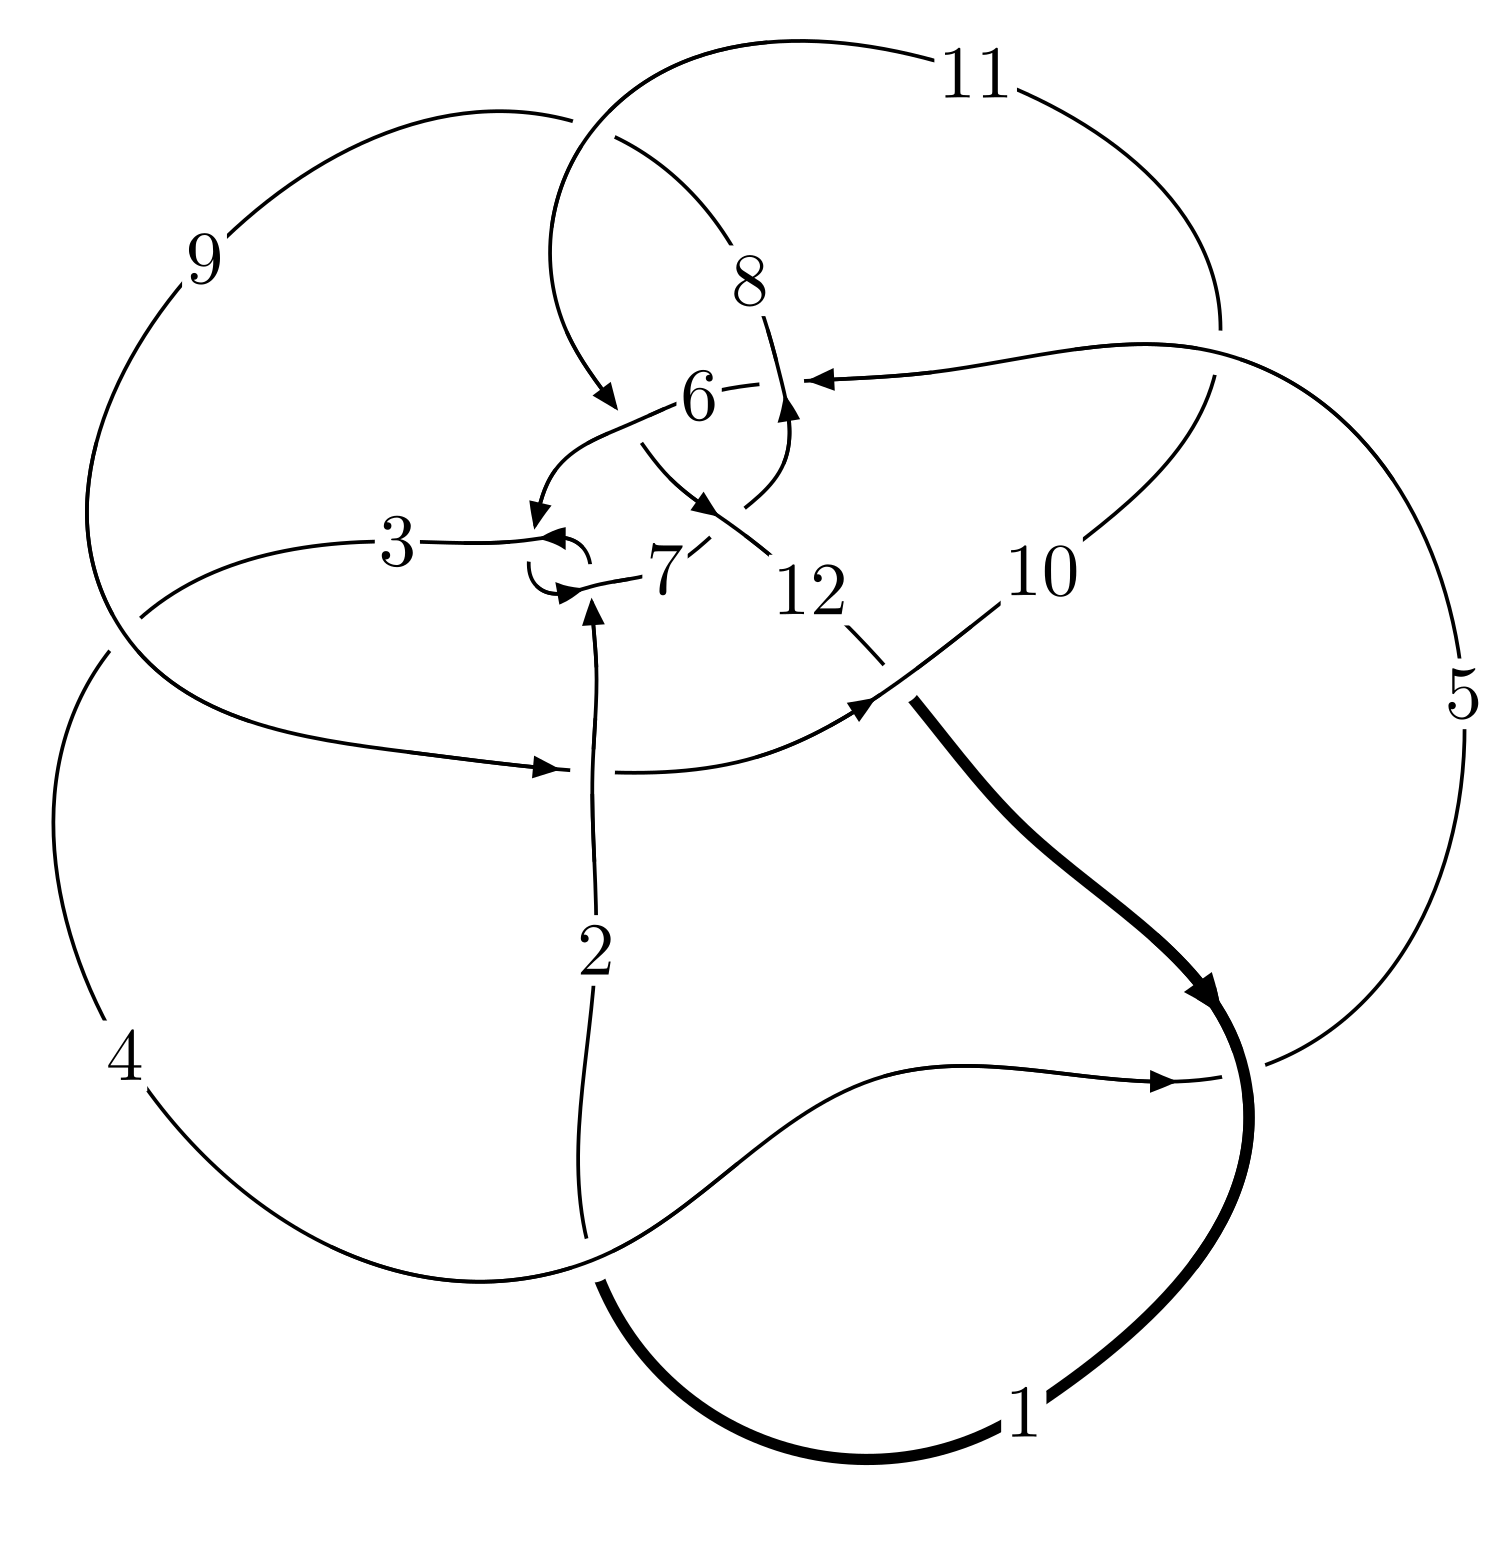
\includegraphics[width=112pt]{../../../GIT/diagram.site/Diagrams/png/1866_12a_1065.png}\\
\ \ \ A knot diagram\footnotemark}&
\allowdisplaybreaks
\textbf{Linearized knot diagam} \\
\cline{2-2}
 &
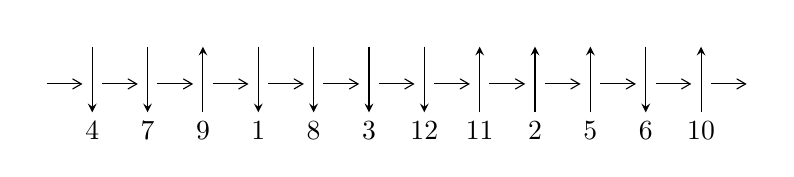
\begin{tikzpicture}[x=20pt, y=17pt]
	% nodes
	\node (C0) at (0, 0) {};
	\node (C1) at (1, 0) {};
	\node (C1U) at (1, +1) {};
	\node (C1D) at (1, -1) {4};

	\node (C2) at (2, 0) {};
	\node (C2U) at (2, +1) {};
	\node (C2D) at (2, -1) {7};

	\node (C3) at (3, 0) {};
	\node (C3U) at (3, +1) {};
	\node (C3D) at (3, -1) {9};

	\node (C4) at (4, 0) {};
	\node (C4U) at (4, +1) {};
	\node (C4D) at (4, -1) {1};

	\node (C5) at (5, 0) {};
	\node (C5U) at (5, +1) {};
	\node (C5D) at (5, -1) {8};

	\node (C6) at (6, 0) {};
	\node (C6U) at (6, +1) {};
	\node (C6D) at (6, -1) {3};

	\node (C7) at (7, 0) {};
	\node (C7U) at (7, +1) {};
	\node (C7D) at (7, -1) {12};

	\node (C8) at (8, 0) {};
	\node (C8U) at (8, +1) {};
	\node (C8D) at (8, -1) {11};

	\node (C9) at (9, 0) {};
	\node (C9U) at (9, +1) {};
	\node (C9D) at (9, -1) {2};

	\node (C10) at (10, 0) {};
	\node (C10U) at (10, +1) {};
	\node (C10D) at (10, -1) {5};

	\node (C11) at (11, 0) {};
	\node (C11U) at (11, +1) {};
	\node (C11D) at (11, -1) {6};

	\node (C12) at (12, 0) {};
	\node (C12U) at (12, +1) {};
	\node (C12D) at (12, -1) {10};
	\node (C13) at (13, 0) {};

	% arrows
	\draw[->,>={angle 60}]
	(C0) edge (C1) (C1) edge (C2) (C2) edge (C3) (C3) edge (C4) (C4) edge (C5) (C5) edge (C6) (C6) edge (C7) (C7) edge (C8) (C8) edge (C9) (C9) edge (C10) (C10) edge (C11) (C11) edge (C12) (C12) edge (C13) ;	\draw[->,>=stealth]
	(C1U) edge (C1D) (C2U) edge (C2D) (C3D) edge (C3U) (C4U) edge (C4D) (C5U) edge (C5D) (C6U) edge (C6D) (C7U) edge (C7D) (C8D) edge (C8U) (C9D) edge (C9U) (C10D) edge (C10U) (C11U) edge (C11D) (C12D) edge (C12U) ;
	\end{tikzpicture} \\
\hhline{~~} \\& 
\textbf{Solving Sequence} \\ \cline{2-2} 
 &
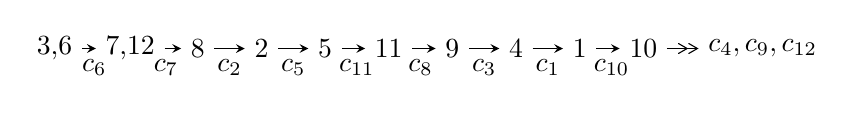
\begin{tikzpicture}[x=23pt, y=7pt]
	% node
	\node (A0) at (-1/8, 0) {3,6};
	\node (A1) at (17/16, 0) {7,12};
	\node (A2) at (17/8, 0) {8};
	\node (A3) at (25/8, 0) {2};
	\node (A4) at (33/8, 0) {5};
	\node (A5) at (41/8, 0) {11};
	\node (A6) at (49/8, 0) {9};
	\node (A7) at (57/8, 0) {4};
	\node (A8) at (65/8, 0) {1};
	\node (A9) at (73/8, 0) {10};
	\node (C1) at (1/2, -1) {$c_{6}$};
	\node (C2) at (13/8, -1) {$c_{7}$};
	\node (C3) at (21/8, -1) {$c_{2}$};
	\node (C4) at (29/8, -1) {$c_{5}$};
	\node (C5) at (37/8, -1) {$c_{11}$};
	\node (C6) at (45/8, -1) {$c_{8}$};
	\node (C7) at (53/8, -1) {$c_{3}$};
	\node (C8) at (61/8, -1) {$c_{1}$};
	\node (C9) at (69/8, -1) {$c_{10}$};
	\node (A10) at (11, 0) {$c_{4},c_{9},c_{12}$};

	% edge
	\draw[->,>=stealth]	
	(A0) edge (A1) (A1) edge (A2) (A2) edge (A3) (A3) edge (A4) (A4) edge (A5) (A5) edge (A6) (A6) edge (A7) (A7) edge (A8) (A8) edge (A9) ;
	\draw[->>,>={angle 60}]	
	(A9) edge (A10);
\end{tikzpicture} \\ 

\end{tabular} \\

\footnotetext{
The image of knot diagram is generated by the software ``\textbf{Draw programme}" developed by Andrew Bartholomew(\url{http://www.layer8.co.uk/maths/draw/index.htm\#Running-draw}), where we modified some parts for our purpose(\url{https://github.com/CATsTAILs/LinksPainter}).
}\phantom \\ \newline 
\centering \textbf{Ideals for irreducible components\footnotemark of $X_{\text{par}}$} 
 
\begin{align*}
I^u_{1}&=\langle 
6.60026\times10^{1371} u^{205}+1.40844\times10^{1372} u^{204}+\cdots+4.43512\times10^{1372} b-7.21056\times10^{1376},\\
\phantom{I^u_{1}}&\phantom{= \langle  }1.27492\times10^{1377} u^{205}+4.66649\times10^{1376} u^{204}+\cdots+1.02057\times10^{1377} a-1.52758\times10^{1381},\\
\phantom{I^u_{1}}&\phantom{= \langle  }u^{206}+50 u^{204}+\cdots+14240 u-23011\rangle \\
I^u_{2}&=\langle 
-2.24645\times10^{57} u^{55}+3.87827\times10^{56} u^{54}+\cdots+9.69748\times10^{54} b+6.73301\times10^{57},\\
\phantom{I^u_{2}}&\phantom{= \langle  }-4.34769\times10^{57} u^{55}+9.99420\times10^{57} u^{54}+\cdots+9.69748\times10^{54} a-3.76270\times10^{58},\;u^{56}- u^{55}+\cdots+u-1\rangle \\
\\
\end{align*}
\raggedright * 2 irreducible components of $\dim_{\mathbb{C}}=0$, with total 262 representations.\\
\footnotetext{All coefficients of polynomials are rational numbers. But the coefficients are sometimes approximated in decimal forms when there is not enough margin.}
\newpage
\renewcommand{\arraystretch}{1}
\centering \section*{I. $I^u_{1}= \langle 6.60\times10^{1371} u^{205}+1.41\times10^{1372} u^{204}+\cdots+4.44\times10^{1372} b-7.21\times10^{1376},\;1.27\times10^{1377} u^{205}+4.67\times10^{1376} u^{204}+\cdots+1.02\times10^{1377} a-1.53\times10^{1381},\;u^{206}+50 u^{204}+\cdots+14240 u-23011 \rangle$}
\flushleft \textbf{(i) Arc colorings}\\
\begin{tabular}{m{7pt} m{180pt} m{7pt} m{180pt} }
\flushright $a_{3}=$&$\begin{pmatrix}0\\u\end{pmatrix}$ \\
\flushright $a_{6}=$&$\begin{pmatrix}1\\0\end{pmatrix}$ \\
\flushright $a_{7}=$&$\begin{pmatrix}1\\u^2\end{pmatrix}$ \\
\flushright $a_{12}=$&$\begin{pmatrix}-1.24923 u^{205}-0.457245 u^{204}+\cdots+49046.6 u+14968.0\\-0.148818 u^{205}-0.317566 u^{204}+\cdots-1675.80 u+16257.9\end{pmatrix}$ \\
\flushright $a_{8}=$&$\begin{pmatrix}2.07913 u^{205}+2.01660 u^{204}+\cdots-54117.4 u-89525.8\\-0.387228 u^{205}+0.221741 u^{204}+\cdots+22547.3 u-12920.9\end{pmatrix}$ \\
\flushright $a_{2}=$&$\begin{pmatrix}u\\u^3+u\end{pmatrix}$ \\
\flushright $a_{5}=$&$\begin{pmatrix}-0.835289 u^{205}-1.85164 u^{204}+\cdots+2325.95 u+84466.1\\0.403162 u^{205}-0.455726 u^{204}+\cdots-26105.0 u+23498.0\end{pmatrix}$ \\
\flushright $a_{11}=$&$\begin{pmatrix}-1.39805 u^{205}-0.774811 u^{204}+\cdots+47370.8 u+31225.8\\-0.148818 u^{205}-0.317566 u^{204}+\cdots-1675.80 u+16257.9\end{pmatrix}$ \\
\flushright $a_{9}=$&$\begin{pmatrix}-0.112651 u^{205}+0.795357 u^{204}+\cdots+18504.6 u-39304.5\\-0.566387 u^{205}+0.141147 u^{204}+\cdots+27229.9 u-8443.97\end{pmatrix}$ \\
\flushright $a_{4}=$&$\begin{pmatrix}1.71560 u^{205}+1.16243 u^{204}+\cdots-55839.1 u-50267.9\\0.0904229 u^{205}-0.118107 u^{204}+\cdots-5227.31 u+5260.12\end{pmatrix}$ \\
\flushright $a_{1}=$&$\begin{pmatrix}-1.02977 u^{205}-2.13736 u^{204}+\cdots+1410.29 u+94281.4\\0.560273 u^{205}-0.495833 u^{204}+\cdots-39580.4 u+26176.1\end{pmatrix}$ \\
\flushright $a_{10}=$&$\begin{pmatrix}0.190370 u^{205}+0.948223 u^{204}+\cdots+8284.65 u-46005.8\\-0.415373 u^{205}+0.213807 u^{204}+\cdots+21806.0 u-11627.6\end{pmatrix}$\\&\end{tabular}
\flushleft \textbf{(ii) Obstruction class $= -1$}\\~\\
\flushleft \textbf{(iii) Cusp Shapes $= -4.45801 u^{205}-3.78212 u^{204}+\cdots+131136. u+149244.$}\\~\\
\newpage\renewcommand{\arraystretch}{1}
\flushleft \textbf{(iv) u-Polynomials at the component}\newline \\
\begin{tabular}{m{50pt}|m{274pt}}
Crossings & \hspace{64pt}u-Polynomials at each crossing \\
\hline $$\begin{aligned}c_{1},c_{4}\end{aligned}$$&$\begin{aligned}
&u^{206}-4 u^{205}+\cdots-6646 u+279
\end{aligned}$\\
\hline $$\begin{aligned}c_{2},c_{6}\end{aligned}$$&$\begin{aligned}
&u^{206}+50 u^{204}+\cdots-14240 u-23011
\end{aligned}$\\
\hline $$\begin{aligned}c_{3}\end{aligned}$$&$\begin{aligned}
&u^{206}-23 u^{204}+\cdots+680803696640 u-49121591296
\end{aligned}$\\
\hline $$\begin{aligned}c_{5}\end{aligned}$$&$\begin{aligned}
&u^{206}-12 u^{205}+\cdots+188 u-8
\end{aligned}$\\
\hline $$\begin{aligned}c_{7}\end{aligned}$$&$\begin{aligned}
&u^{206}-7 u^{204}+\cdots+307888522 u-10416143
\end{aligned}$\\
\hline $$\begin{aligned}c_{8}\end{aligned}$$&$\begin{aligned}
&u^{206}-14 u^{205}+\cdots+82275 u+1921
\end{aligned}$\\
\hline $$\begin{aligned}c_{9}\end{aligned}$$&$\begin{aligned}
&u^{206}-3 u^{205}+\cdots+549559 u-340933
\end{aligned}$\\
\hline $$\begin{aligned}c_{10}\end{aligned}$$&$\begin{aligned}
&u^{206}-2 u^{205}+\cdots-252875824155 u-41030919307
\end{aligned}$\\
\hline $$\begin{aligned}c_{11}\end{aligned}$$&$\begin{aligned}
&u^{206}-4 u^{205}+\cdots-85 u+3
\end{aligned}$\\
\hline $$\begin{aligned}c_{12}\end{aligned}$$&$\begin{aligned}
&u^{206}-12 u^{205}+\cdots-1031021376 u-198007488
\end{aligned}$\\
\hline
\end{tabular}\\~\\
\newpage\renewcommand{\arraystretch}{1}
\flushleft \textbf{(v) Riley Polynomials at the component}\newline \\
\begin{tabular}{m{50pt}|m{274pt}}
Crossings & \hspace{64pt}Riley Polynomials at each crossing \\
\hline $$\begin{aligned}c_{1},c_{4}\end{aligned}$$&$\begin{aligned}
&y^{206}+142 y^{205}+\cdots+261434 y+77841
\end{aligned}$\\
\hline $$\begin{aligned}c_{2},c_{6}\end{aligned}$$&$\begin{aligned}
&y^{206}+100 y^{205}+\cdots+27689085610 y+529506121
\end{aligned}$\\
\hline $$\begin{aligned}c_{3}\end{aligned}$$&$\begin{aligned}
&y^{206}-46 y^{205}+\cdots-1.93\times10^{23} y+2.41\times10^{21}
\end{aligned}$\\
\hline $$\begin{aligned}c_{5}\end{aligned}$$&$\begin{aligned}
&y^{206}+2 y^{205}+\cdots+9776 y+64
\end{aligned}$\\
\hline $$\begin{aligned}c_{7}\end{aligned}$$&$\begin{aligned}
&y^{206}-14 y^{205}+\cdots+8508975757402814 y+108496034996449
\end{aligned}$\\
\hline $$\begin{aligned}c_{8}\end{aligned}$$&$\begin{aligned}
&y^{206}-36 y^{205}+\cdots-4238192811 y+3690241
\end{aligned}$\\
\hline $$\begin{aligned}c_{9}\end{aligned}$$&$\begin{aligned}
&y^{206}-21 y^{205}+\cdots-16612307091225 y+116235310489
\end{aligned}$\\
\hline $$\begin{aligned}c_{10}\end{aligned}$$&$\begin{aligned}
&y^{206}-98 y^{205}+\cdots-1.61\times10^{23} y+1.68\times10^{21}
\end{aligned}$\\
\hline $$\begin{aligned}c_{11}\end{aligned}$$&$\begin{aligned}
&y^{206}-10 y^{205}+\cdots-283 y+9
\end{aligned}$\\
\hline $$\begin{aligned}c_{12}\end{aligned}$$&$\begin{aligned}
&y^{206}-60 y^{205}+\cdots-3145705022699527680 y+39206965304070144
\end{aligned}$\\
\hline
\end{tabular}\\~\\
\newpage\flushleft \textbf{(vi) Complex Volumes and Cusp Shapes}
$$\begin{array}{c|c|c}  
\text{Solutions to }I^u_{1}& \I (\text{vol} + \sqrt{-1}CS) & \text{Cusp shape}\\
 \hline 
\begin{aligned}
u &= -0.852378 + 0.499579 I \\
a &= \phantom{-}0.221394 + 0.192372 I \\
b &= -0.462433 + 0.321891 I\end{aligned}
 & \phantom{-}3.63058 + 3.34731 I & \phantom{-0.000000 } 0 \\ \hline\begin{aligned}
u &= -0.852378 - 0.499579 I \\
a &= \phantom{-}0.221394 - 0.192372 I \\
b &= -0.462433 - 0.321891 I\end{aligned}
 & \phantom{-}3.63058 - 3.34731 I & \phantom{-0.000000 } 0 \\ \hline\begin{aligned}
u &= \phantom{-}0.415178 + 0.924701 I \\
a &= -1.37433 + 1.15611 I \\
b &= -0.210343 - 0.935141 I\end{aligned}
 & \phantom{-}6.62024 - 5.22982 I & \phantom{-0.000000 } 0 \\ \hline\begin{aligned}
u &= \phantom{-}0.415178 - 0.924701 I \\
a &= -1.37433 - 1.15611 I \\
b &= -0.210343 + 0.935141 I\end{aligned}
 & \phantom{-}6.62024 + 5.22982 I & \phantom{-0.000000 } 0 \\ \hline\begin{aligned}
u &= \phantom{-}0.648840 + 0.789093 I \\
a &= \phantom{-}0.362405 - 0.696253 I \\
b &= \phantom{-}0.025672 - 0.202908 I\end{aligned}
 & \phantom{-}4.12915 + 0.21751 I & \phantom{-0.000000 } 0 \\ \hline\begin{aligned}
u &= \phantom{-}0.648840 - 0.789093 I \\
a &= \phantom{-}0.362405 + 0.696253 I \\
b &= \phantom{-}0.025672 + 0.202908 I\end{aligned}
 & \phantom{-}4.12915 - 0.21751 I & \phantom{-0.000000 } 0 \\ \hline\begin{aligned}
u &= -0.299755 + 0.985648 I \\
a &= \phantom{-}0.17545 + 1.94630 I \\
b &= -0.081399 - 1.132500 I\end{aligned}
 & \phantom{-}4.18133 + 0.96771 I & \phantom{-0.000000 } 0 \\ \hline\begin{aligned}
u &= -0.299755 - 0.985648 I \\
a &= \phantom{-}0.17545 - 1.94630 I \\
b &= -0.081399 + 1.132500 I\end{aligned}
 & \phantom{-}4.18133 - 0.96771 I & \phantom{-0.000000 } 0 \\ \hline\begin{aligned}
u &= -0.247149 + 1.010070 I \\
a &= -1.42325 - 1.58111 I \\
b &= \phantom{-}0.48621 + 1.68214 I\end{aligned}
 & \phantom{-}8.65376 + 0.73150 I & \phantom{-0.000000 } 0 \\ \hline\begin{aligned}
u &= -0.247149 - 1.010070 I \\
a &= -1.42325 + 1.58111 I \\
b &= \phantom{-}0.48621 - 1.68214 I\end{aligned}
 & \phantom{-}8.65376 - 0.73150 I & \phantom{-0.000000 } 0\\
 \hline 
 \end{array}$$\newpage$$\begin{array}{c|c|c}  
\text{Solutions to }I^u_{1}& \I (\text{vol} + \sqrt{-1}CS) & \text{Cusp shape}\\
 \hline 
\begin{aligned}
u &= \phantom{-}0.196900 + 1.039640 I \\
a &= -0.27451 - 1.91756 I \\
b &= -0.099253 + 1.145380 I\end{aligned}
 & \phantom{-}8.78142 - 0.45494 I & \phantom{-0.000000 } 0 \\ \hline\begin{aligned}
u &= \phantom{-}0.196900 - 1.039640 I \\
a &= -0.27451 + 1.91756 I \\
b &= -0.099253 - 1.145380 I\end{aligned}
 & \phantom{-}8.78142 + 0.45494 I & \phantom{-0.000000 } 0 \\ \hline\begin{aligned}
u &= -0.919057 + 0.524548 I \\
a &= -0.507244 + 0.608003 I \\
b &= -0.270865 + 0.186214 I\end{aligned}
 & \phantom{-}0.27564 + 5.22638 I & \phantom{-0.000000 } 0 \\ \hline\begin{aligned}
u &= -0.919057 - 0.524548 I \\
a &= -0.507244 - 0.608003 I \\
b &= -0.270865 - 0.186214 I\end{aligned}
 & \phantom{-}0.27564 - 5.22638 I & \phantom{-0.000000 } 0 \\ \hline\begin{aligned}
u &= -0.011444 + 0.936367 I \\
a &= -1.92823 + 1.05959 I \\
b &= \phantom{-}2.26010 - 0.55093 I\end{aligned}
 & \phantom{-}4.64921 + 0.77443 I & \phantom{-0.000000 } 0 \\ \hline\begin{aligned}
u &= -0.011444 - 0.936367 I \\
a &= -1.92823 - 1.05959 I \\
b &= \phantom{-}2.26010 + 0.55093 I\end{aligned}
 & \phantom{-}4.64921 - 0.77443 I & \phantom{-0.000000 } 0 \\ \hline\begin{aligned}
u &= \phantom{-}0.121941 + 1.056860 I \\
a &= -0.98991 + 2.05783 I \\
b &= \phantom{-}0.55495 - 2.05384 I\end{aligned}
 & \phantom{-}4.18537 - 0.25383 I & \phantom{-0.000000 } 0 \\ \hline\begin{aligned}
u &= \phantom{-}0.121941 - 1.056860 I \\
a &= -0.98991 - 2.05783 I \\
b &= \phantom{-}0.55495 + 2.05384 I\end{aligned}
 & \phantom{-}4.18537 + 0.25383 I & \phantom{-0.000000 } 0 \\ \hline\begin{aligned}
u &= \phantom{-}0.914468 + 0.197123 I \\
a &= -0.047993 - 0.236538 I \\
b &= -0.746350 - 0.718300 I\end{aligned}
 & \phantom{-}2.76022 - 6.79685 I & \phantom{-0.000000 } 0 \\ \hline\begin{aligned}
u &= \phantom{-}0.914468 - 0.197123 I \\
a &= -0.047993 + 0.236538 I \\
b &= -0.746350 + 0.718300 I\end{aligned}
 & \phantom{-}2.76022 + 6.79685 I & \phantom{-0.000000 } 0\\
 \hline 
 \end{array}$$\newpage$$\begin{array}{c|c|c}  
\text{Solutions to }I^u_{1}& \I (\text{vol} + \sqrt{-1}CS) & \text{Cusp shape}\\
 \hline 
\begin{aligned}
u &= -0.816119 + 0.426958 I \\
a &= \phantom{-}1.077320 + 0.791595 I \\
b &= \phantom{-}0.868748 - 0.888779 I\end{aligned}
 & \phantom{-}4.24470 + 4.76496 I & \phantom{-0.000000 } 0 \\ \hline\begin{aligned}
u &= -0.816119 - 0.426958 I \\
a &= \phantom{-}1.077320 - 0.791595 I \\
b &= \phantom{-}0.868748 + 0.888779 I\end{aligned}
 & \phantom{-}4.24470 - 4.76496 I & \phantom{-0.000000 } 0 \\ \hline\begin{aligned}
u &= \phantom{-}0.279578 + 0.866302 I \\
a &= \phantom{-}0.42576 + 2.75431 I \\
b &= -1.07454 - 1.15296 I\end{aligned}
 & -0.0946138 + 0.0931659 I & \phantom{-0.000000 } 0 \\ \hline\begin{aligned}
u &= \phantom{-}0.279578 - 0.866302 I \\
a &= \phantom{-}0.42576 - 2.75431 I \\
b &= -1.07454 + 1.15296 I\end{aligned}
 & -0.0946138 - 0.0931659 I & \phantom{-0.000000 } 0 \\ \hline\begin{aligned}
u &= \phantom{-}0.380299 + 1.022350 I \\
a &= \phantom{-}0.67042 - 1.95304 I \\
b &= \phantom{-}0.13729 + 1.53736 I\end{aligned}
 & \phantom{-}6.87881 - 0.71094 I & \phantom{-0.000000 } 0 \\ \hline\begin{aligned}
u &= \phantom{-}0.380299 - 1.022350 I \\
a &= \phantom{-}0.67042 + 1.95304 I \\
b &= \phantom{-}0.13729 - 1.53736 I\end{aligned}
 & \phantom{-}6.87881 + 0.71094 I & \phantom{-0.000000 } 0 \\ \hline\begin{aligned}
u &= -0.384170 + 0.817717 I \\
a &= -0.15915 - 2.83800 I \\
b &= -0.89962 + 1.09241 I\end{aligned}
 & -3.10470 + 4.33797 I & \phantom{-0.000000 } 0 \\ \hline\begin{aligned}
u &= -0.384170 - 0.817717 I \\
a &= -0.15915 + 2.83800 I \\
b &= -0.89962 - 1.09241 I\end{aligned}
 & -3.10470 - 4.33797 I & \phantom{-0.000000 } 0 \\ \hline\begin{aligned}
u &= -1.077140 + 0.218578 I \\
a &= -0.002824 - 0.315354 I \\
b &= -0.832742 - 0.964996 I\end{aligned}
 & -1.02001 - 6.68521 I & \phantom{-0.000000 } 0 \\ \hline\begin{aligned}
u &= -1.077140 - 0.218578 I \\
a &= -0.002824 + 0.315354 I \\
b &= -0.832742 + 0.964996 I\end{aligned}
 & -1.02001 + 6.68521 I & \phantom{-0.000000 } 0\\
 \hline 
 \end{array}$$\newpage$$\begin{array}{c|c|c}  
\text{Solutions to }I^u_{1}& \I (\text{vol} + \sqrt{-1}CS) & \text{Cusp shape}\\
 \hline 
\begin{aligned}
u &= \phantom{-}0.265527 + 0.859681 I \\
a &= -0.546821 + 0.022818 I \\
b &= \phantom{-}1.51083 - 0.58470 I\end{aligned}
 & -0.14831 - 2.62345 I & \phantom{-0.000000 } 0 \\ \hline\begin{aligned}
u &= \phantom{-}0.265527 - 0.859681 I \\
a &= -0.546821 - 0.022818 I \\
b &= \phantom{-}1.51083 + 0.58470 I\end{aligned}
 & -0.14831 + 2.62345 I & \phantom{-0.000000 } 0 \\ \hline\begin{aligned}
u &= \phantom{-}0.609674 + 0.644447 I \\
a &= \phantom{-}0.194304 + 0.179284 I \\
b &= -0.991421 - 0.189066 I\end{aligned}
 & -1.57551 - 5.11041 I & \phantom{-0.000000 } 0 \\ \hline\begin{aligned}
u &= \phantom{-}0.609674 - 0.644447 I \\
a &= \phantom{-}0.194304 - 0.179284 I \\
b &= -0.991421 + 0.189066 I\end{aligned}
 & -1.57551 + 5.11041 I & \phantom{-0.000000 } 0 \\ \hline\begin{aligned}
u &= \phantom{-}1.112390 + 0.107441 I \\
a &= \phantom{-}0.284219 - 0.318587 I \\
b &= -0.252935 - 0.027578 I\end{aligned}
 & -2.61789 + 0.31689 I & \phantom{-0.000000 } 0 \\ \hline\begin{aligned}
u &= \phantom{-}1.112390 - 0.107441 I \\
a &= \phantom{-}0.284219 + 0.318587 I \\
b &= -0.252935 + 0.027578 I\end{aligned}
 & -2.61789 - 0.31689 I & \phantom{-0.000000 } 0 \\ \hline\begin{aligned}
u &= -0.107963 + 1.115960 I \\
a &= \phantom{-}0.81574 + 1.88221 I \\
b &= -0.88592 - 2.14946 I\end{aligned}
 & \phantom{-}4.58557 - 0.30273 I & \phantom{-0.000000 } 0 \\ \hline\begin{aligned}
u &= -0.107963 - 1.115960 I \\
a &= \phantom{-}0.81574 - 1.88221 I \\
b &= -0.88592 + 2.14946 I\end{aligned}
 & \phantom{-}4.58557 + 0.30273 I & \phantom{-0.000000 } 0 \\ \hline\begin{aligned}
u &= -0.476820 + 1.021780 I \\
a &= \phantom{-}0.404735 + 1.165530 I \\
b &= \phantom{-}0.142026 - 0.170506 I\end{aligned}
 & \phantom{-}2.29162 - 0.22801 I & \phantom{-0.000000 } 0 \\ \hline\begin{aligned}
u &= -0.476820 - 1.021780 I \\
a &= \phantom{-}0.404735 - 1.165530 I \\
b &= \phantom{-}0.142026 + 0.170506 I\end{aligned}
 & \phantom{-}2.29162 + 0.22801 I & \phantom{-0.000000 } 0\\
 \hline 
 \end{array}$$\newpage$$\begin{array}{c|c|c}  
\text{Solutions to }I^u_{1}& \I (\text{vol} + \sqrt{-1}CS) & \text{Cusp shape}\\
 \hline 
\begin{aligned}
u &= \phantom{-}0.358266 + 1.074370 I \\
a &= -1.29758 + 0.75212 I \\
b &= \phantom{-}0.71239 - 1.32851 I\end{aligned}
 & \phantom{-}7.42750 + 3.00839 I & \phantom{-0.000000 } 0 \\ \hline\begin{aligned}
u &= \phantom{-}0.358266 - 1.074370 I \\
a &= -1.29758 - 0.75212 I \\
b &= \phantom{-}0.71239 + 1.32851 I\end{aligned}
 & \phantom{-}7.42750 - 3.00839 I & \phantom{-0.000000 } 0 \\ \hline\begin{aligned}
u &= \phantom{-}0.759917 + 0.412152 I \\
a &= \phantom{-}1.67316 - 0.72560 I \\
b &= \phantom{-}0.923789 - 0.335686 I\end{aligned}
 & -1.57514 - 2.05589 I & \phantom{-0.000000 } 0 \\ \hline\begin{aligned}
u &= \phantom{-}0.759917 - 0.412152 I \\
a &= \phantom{-}1.67316 + 0.72560 I \\
b &= \phantom{-}0.923789 + 0.335686 I\end{aligned}
 & -1.57514 + 2.05589 I & \phantom{-0.000000 } 0 \\ \hline\begin{aligned}
u &= -0.403296 + 0.759359 I \\
a &= -0.160593 - 0.156643 I \\
b &= \phantom{-}1.231220 + 0.608968 I\end{aligned}
 & -3.24962 - 0.85600 I & \phantom{-0.000000 } 0 \\ \hline\begin{aligned}
u &= -0.403296 - 0.759359 I \\
a &= -0.160593 + 0.156643 I \\
b &= \phantom{-}1.231220 - 0.608968 I\end{aligned}
 & -3.24962 + 0.85600 I & \phantom{-0.000000 } 0 \\ \hline\begin{aligned}
u &= -0.456692 + 1.049510 I \\
a &= \phantom{-}0.403526 + 1.281480 I \\
b &= \phantom{-}0.150743 - 0.224019 I\end{aligned}
 & \phantom{-}2.29639 - 0.22767 I & \phantom{-0.000000 } 0 \\ \hline\begin{aligned}
u &= -0.456692 - 1.049510 I \\
a &= \phantom{-}0.403526 - 1.281480 I \\
b &= \phantom{-}0.150743 + 0.224019 I\end{aligned}
 & \phantom{-}2.29639 + 0.22767 I & \phantom{-0.000000 } 0 \\ \hline\begin{aligned}
u &= \phantom{-}0.915348 + 0.694450 I \\
a &= \phantom{-}0.104046 - 0.419376 I \\
b &= \phantom{-}0.569474 + 0.310786 I\end{aligned}
 & -1.227550 - 0.435334 I & \phantom{-0.000000 } 0 \\ \hline\begin{aligned}
u &= \phantom{-}0.915348 - 0.694450 I \\
a &= \phantom{-}0.104046 + 0.419376 I \\
b &= \phantom{-}0.569474 - 0.310786 I\end{aligned}
 & -1.227550 + 0.435334 I & \phantom{-0.000000 } 0\\
 \hline 
 \end{array}$$\newpage$$\begin{array}{c|c|c}  
\text{Solutions to }I^u_{1}& \I (\text{vol} + \sqrt{-1}CS) & \text{Cusp shape}\\
 \hline 
\begin{aligned}
u &= \phantom{-}0.532731 + 1.025950 I \\
a &= -0.885459 + 0.487937 I \\
b &= -0.859686 + 0.034392 I\end{aligned}
 & \phantom{-}0.12635 - 2.70025 I & \phantom{-0.000000 } 0 \\ \hline\begin{aligned}
u &= \phantom{-}0.532731 - 1.025950 I \\
a &= -0.885459 - 0.487937 I \\
b &= -0.859686 - 0.034392 I\end{aligned}
 & \phantom{-}0.12635 + 2.70025 I & \phantom{-0.000000 } 0 \\ \hline\begin{aligned}
u &= -0.107066 + 0.833430 I \\
a &= \phantom{-}1.334520 + 0.048843 I \\
b &= -1.31665 - 0.52950 I\end{aligned}
 & \phantom{-}4.62180 - 0.51584 I & \phantom{-0.000000 } 0 \\ \hline\begin{aligned}
u &= -0.107066 - 0.833430 I \\
a &= \phantom{-}1.334520 - 0.048843 I \\
b &= -1.31665 + 0.52950 I\end{aligned}
 & \phantom{-}4.62180 + 0.51584 I & \phantom{-0.000000 } 0 \\ \hline\begin{aligned}
u &= -0.665342 + 0.952042 I \\
a &= -0.904490 - 0.486367 I \\
b &= -0.402480 + 0.491378 I\end{aligned}
 & \phantom{-}2.05534 + 4.67725 I & \phantom{-0.000000 } 0 \\ \hline\begin{aligned}
u &= -0.665342 - 0.952042 I \\
a &= -0.904490 + 0.486367 I \\
b &= -0.402480 - 0.491378 I\end{aligned}
 & \phantom{-}2.05534 - 4.67725 I & \phantom{-0.000000 } 0 \\ \hline\begin{aligned}
u &= \phantom{-}0.826394 + 0.127642 I \\
a &= \phantom{-}0.361916 + 0.024212 I \\
b &= \phantom{-}0.950630 - 0.523871 I\end{aligned}
 & -0.98212 + 1.37040 I & \phantom{-0.000000 } 0 \\ \hline\begin{aligned}
u &= \phantom{-}0.826394 - 0.127642 I \\
a &= \phantom{-}0.361916 - 0.024212 I \\
b &= \phantom{-}0.950630 + 0.523871 I\end{aligned}
 & -0.98212 - 1.37040 I & \phantom{-0.000000 } 0 \\ \hline\begin{aligned}
u &= -0.419673 + 0.717810 I \\
a &= \phantom{-}0.137164 - 0.568619 I \\
b &= -1.269710 + 0.347068 I\end{aligned}
 & \phantom{-}1.39966 + 8.61799 I & \phantom{-0.000000 } 0 \\ \hline\begin{aligned}
u &= -0.419673 - 0.717810 I \\
a &= \phantom{-}0.137164 + 0.568619 I \\
b &= -1.269710 - 0.347068 I\end{aligned}
 & \phantom{-}1.39966 - 8.61799 I & \phantom{-0.000000 } 0\\
 \hline 
 \end{array}$$\newpage$$\begin{array}{c|c|c}  
\text{Solutions to }I^u_{1}& \I (\text{vol} + \sqrt{-1}CS) & \text{Cusp shape}\\
 \hline 
\begin{aligned}
u &= -0.822934 + 0.081342 I \\
a &= \phantom{-}1.76184 + 0.42924 I \\
b &= \phantom{-}1.039030 + 0.914148 I\end{aligned}
 & \phantom{-}3.99123 + 7.92047 I & \phantom{-0.000000 } 0 \\ \hline\begin{aligned}
u &= -0.822934 - 0.081342 I \\
a &= \phantom{-}1.76184 - 0.42924 I \\
b &= \phantom{-}1.039030 - 0.914148 I\end{aligned}
 & \phantom{-}3.99123 - 7.92047 I & \phantom{-0.000000 } 0 \\ \hline\begin{aligned}
u &= -0.438018 + 1.095550 I \\
a &= \phantom{-}0.01326 + 2.15202 I \\
b &= \phantom{-}1.22517 - 0.83549 I\end{aligned}
 & \phantom{-}3.45836 + 11.03310 I & \phantom{-0.000000 } 0 \\ \hline\begin{aligned}
u &= -0.438018 - 1.095550 I \\
a &= \phantom{-}0.01326 - 2.15202 I \\
b &= \phantom{-}1.22517 + 0.83549 I\end{aligned}
 & \phantom{-}3.45836 - 11.03310 I & \phantom{-0.000000 } 0 \\ \hline\begin{aligned}
u &= -0.707653 + 0.945252 I \\
a &= -0.501513 + 0.431326 I \\
b &= \phantom{-}0.775148 + 0.143708 I\end{aligned}
 & \phantom{-}2.09667 - 4.14322 I & \phantom{-0.000000 } 0 \\ \hline\begin{aligned}
u &= -0.707653 - 0.945252 I \\
a &= -0.501513 - 0.431326 I \\
b &= \phantom{-}0.775148 - 0.143708 I\end{aligned}
 & \phantom{-}2.09667 + 4.14322 I & \phantom{-0.000000 } 0 \\ \hline\begin{aligned}
u &= -0.705918 + 0.415082 I \\
a &= \phantom{-}0.466083 - 0.033394 I \\
b &= \phantom{-}1.055500 + 0.327775 I\end{aligned}
 & -0.250568 - 0.890470 I & \phantom{-0.000000 } 0 \\ \hline\begin{aligned}
u &= -0.705918 - 0.415082 I \\
a &= \phantom{-}0.466083 + 0.033394 I \\
b &= \phantom{-}1.055500 - 0.327775 I\end{aligned}
 & -0.250568 + 0.890470 I & \phantom{-0.000000 } 0 \\ \hline\begin{aligned}
u &= \phantom{-}0.535241 + 0.614850 I \\
a &= -1.28423 + 3.02459 I \\
b &= -0.619608 - 0.936648 I\end{aligned}
 & \phantom{-}2.44673 - 8.59776 I & \phantom{-0.000000 } 0 \\ \hline\begin{aligned}
u &= \phantom{-}0.535241 - 0.614850 I \\
a &= -1.28423 - 3.02459 I \\
b &= -0.619608 + 0.936648 I\end{aligned}
 & \phantom{-}2.44673 + 8.59776 I & \phantom{-0.000000 } 0\\
 \hline 
 \end{array}$$\newpage$$\begin{array}{c|c|c}  
\text{Solutions to }I^u_{1}& \I (\text{vol} + \sqrt{-1}CS) & \text{Cusp shape}\\
 \hline 
\begin{aligned}
u &= -0.033252 + 0.811950 I \\
a &= -1.22833 - 1.92504 I \\
b &= \phantom{-}1.226220 + 0.478441 I\end{aligned}
 & \phantom{-}1.50486 + 2.03777 I & \phantom{-0.000000 } 0 \\ \hline\begin{aligned}
u &= -0.033252 - 0.811950 I \\
a &= -1.22833 + 1.92504 I \\
b &= \phantom{-}1.226220 - 0.478441 I\end{aligned}
 & \phantom{-}1.50486 - 2.03777 I & \phantom{-0.000000 } 0 \\ \hline\begin{aligned}
u &= -0.549754 + 1.054020 I \\
a &= -0.25095 - 1.73819 I \\
b &= -0.981344 + 0.496292 I\end{aligned}
 & \phantom{-}1.58501 + 5.67095 I & \phantom{-0.000000 } 0 \\ \hline\begin{aligned}
u &= -0.549754 - 1.054020 I \\
a &= -0.25095 + 1.73819 I \\
b &= -0.981344 - 0.496292 I\end{aligned}
 & \phantom{-}1.58501 - 5.67095 I & \phantom{-0.000000 } 0 \\ \hline\begin{aligned}
u &= \phantom{-}0.378154 + 1.127360 I \\
a &= \phantom{-}1.16278 - 1.30964 I \\
b &= \phantom{-}0.145935 + 0.401150 I\end{aligned}
 & \phantom{-}8.21574 + 3.38820 I & \phantom{-0.000000 } 0 \\ \hline\begin{aligned}
u &= \phantom{-}0.378154 - 1.127360 I \\
a &= \phantom{-}1.16278 + 1.30964 I \\
b &= \phantom{-}0.145935 - 0.401150 I\end{aligned}
 & \phantom{-}8.21574 - 3.38820 I & \phantom{-0.000000 } 0 \\ \hline\begin{aligned}
u &= -0.524164 + 1.070540 I \\
a &= -0.805203 - 1.019350 I \\
b &= -0.831685 + 0.534672 I\end{aligned}
 & \phantom{-}2.58286 + 7.16096 I & \phantom{-0.000000 } 0 \\ \hline\begin{aligned}
u &= -0.524164 - 1.070540 I \\
a &= -0.805203 + 1.019350 I \\
b &= -0.831685 - 0.534672 I\end{aligned}
 & \phantom{-}2.58286 - 7.16096 I & \phantom{-0.000000 } 0 \\ \hline\begin{aligned}
u &= \phantom{-}0.421647 + 1.115260 I \\
a &= \phantom{-}1.42759 + 0.15198 I \\
b &= \phantom{-}0.719870 + 0.083101 I\end{aligned}
 & \phantom{-}5.27680 - 11.23860 I & \phantom{-0.000000 } 0 \\ \hline\begin{aligned}
u &= \phantom{-}0.421647 - 1.115260 I \\
a &= \phantom{-}1.42759 - 0.15198 I \\
b &= \phantom{-}0.719870 - 0.083101 I\end{aligned}
 & \phantom{-}5.27680 + 11.23860 I & \phantom{-0.000000 } 0\\
 \hline 
 \end{array}$$\newpage$$\begin{array}{c|c|c}  
\text{Solutions to }I^u_{1}& \I (\text{vol} + \sqrt{-1}CS) & \text{Cusp shape}\\
 \hline 
\begin{aligned}
u &= \phantom{-}0.375545 + 1.138710 I \\
a &= -0.24375 - 2.01328 I \\
b &= \phantom{-}0.935732 + 0.798136 I\end{aligned}
 & \phantom{-}2.12136 - 7.40092 I & \phantom{-0.000000 } 0 \\ \hline\begin{aligned}
u &= \phantom{-}0.375545 - 1.138710 I \\
a &= -0.24375 + 2.01328 I \\
b &= \phantom{-}0.935732 - 0.798136 I\end{aligned}
 & \phantom{-}2.12136 + 7.40092 I & \phantom{-0.000000 } 0 \\ \hline\begin{aligned}
u &= \phantom{-}1.200120 + 0.041594 I \\
a &= \phantom{-}1.092250 + 0.248745 I \\
b &= \phantom{-}1.17798 + 1.27007 I\end{aligned}
 & -1.02024 + 1.69563 I & \phantom{-0.000000 } 0 \\ \hline\begin{aligned}
u &= \phantom{-}1.200120 - 0.041594 I \\
a &= \phantom{-}1.092250 - 0.248745 I \\
b &= \phantom{-}1.17798 - 1.27007 I\end{aligned}
 & -1.02024 - 1.69563 I & \phantom{-0.000000 } 0 \\ \hline\begin{aligned}
u &= \phantom{-}0.167997 + 0.772634 I \\
a &= \phantom{-}1.22340 + 1.97951 I \\
b &= -0.362203 - 0.024099 I\end{aligned}
 & -0.50571 - 2.98010 I & \phantom{-0.000000 } 0 \\ \hline\begin{aligned}
u &= \phantom{-}0.167997 - 0.772634 I \\
a &= \phantom{-}1.22340 - 1.97951 I \\
b &= -0.362203 + 0.024099 I\end{aligned}
 & -0.50571 + 2.98010 I & \phantom{-0.000000 } 0 \\ \hline\begin{aligned}
u &= \phantom{-}0.506674 + 1.102510 I \\
a &= -0.16737 + 1.81510 I \\
b &= -1.076060 - 0.739460 I\end{aligned}
 & \phantom{-}1.74707 - 5.94836 I & \phantom{-0.000000 } 0 \\ \hline\begin{aligned}
u &= \phantom{-}0.506674 - 1.102510 I \\
a &= -0.16737 - 1.81510 I \\
b &= -1.076060 + 0.739460 I\end{aligned}
 & \phantom{-}1.74707 + 5.94836 I & \phantom{-0.000000 } 0 \\ \hline\begin{aligned}
u &= \phantom{-}1.121240 + 0.464967 I \\
a &= \phantom{-}0.088981 + 0.384115 I \\
b &= -0.93261 + 1.20327 I\end{aligned}
 & -2.88716 + 1.88909 I & \phantom{-0.000000 } 0 \\ \hline\begin{aligned}
u &= \phantom{-}1.121240 - 0.464967 I \\
a &= \phantom{-}0.088981 - 0.384115 I \\
b &= -0.93261 - 1.20327 I\end{aligned}
 & -2.88716 - 1.88909 I & \phantom{-0.000000 } 0\\
 \hline 
 \end{array}$$\newpage$$\begin{array}{c|c|c}  
\text{Solutions to }I^u_{1}& \I (\text{vol} + \sqrt{-1}CS) & \text{Cusp shape}\\
 \hline 
\begin{aligned}
u &= -0.526374 + 1.094230 I \\
a &= -0.65069 - 1.85443 I \\
b &= -0.462201 + 0.597448 I\end{aligned}
 & \phantom{-}1.32353 + 7.10432 I & \phantom{-0.000000 } 0 \\ \hline\begin{aligned}
u &= -0.526374 - 1.094230 I \\
a &= -0.65069 + 1.85443 I \\
b &= -0.462201 - 0.597448 I\end{aligned}
 & \phantom{-}1.32353 - 7.10432 I & \phantom{-0.000000 } 0 \\ \hline\begin{aligned}
u &= -0.668922 + 1.020000 I \\
a &= \phantom{-}0.80898 + 1.74359 I \\
b &= \phantom{-}1.25535 - 1.10118 I\end{aligned}
 & \phantom{-}5.84970 + 5.51677 I & \phantom{-0.000000 } 0 \\ \hline\begin{aligned}
u &= -0.668922 - 1.020000 I \\
a &= \phantom{-}0.80898 - 1.74359 I \\
b &= \phantom{-}1.25535 + 1.10118 I\end{aligned}
 & \phantom{-}5.84970 - 5.51677 I & \phantom{-0.000000 } 0 \\ \hline\begin{aligned}
u &= -0.362972 + 1.166880 I \\
a &= -0.05599 - 1.57405 I \\
b &= -1.55200 + 0.63923 I\end{aligned}
 & \phantom{-}8.51017 + 7.88042 I & \phantom{-0.000000 } 0 \\ \hline\begin{aligned}
u &= -0.362972 - 1.166880 I \\
a &= -0.05599 + 1.57405 I \\
b &= -1.55200 - 0.63923 I\end{aligned}
 & \phantom{-}8.51017 - 7.88042 I & \phantom{-0.000000 } 0 \\ \hline\begin{aligned}
u &= \phantom{-}0.476971 + 1.128190 I \\
a &= -0.179142 + 1.118020 I \\
b &= -0.579401 - 0.358466 I\end{aligned}
 & \phantom{-}1.17039 - 3.51010 I & \phantom{-0.000000 } 0 \\ \hline\begin{aligned}
u &= \phantom{-}0.476971 - 1.128190 I \\
a &= -0.179142 - 1.118020 I \\
b &= -0.579401 + 0.358466 I\end{aligned}
 & \phantom{-}1.17039 + 3.51010 I & \phantom{-0.000000 } 0 \\ \hline\begin{aligned}
u &= \phantom{-}0.376067 + 1.168630 I \\
a &= -0.32751 - 1.58525 I \\
b &= \phantom{-}0.411466 + 0.521518 I\end{aligned}
 & \phantom{-}1.62907 - 4.76673 I & \phantom{-0.000000 } 0 \\ \hline\begin{aligned}
u &= \phantom{-}0.376067 - 1.168630 I \\
a &= -0.32751 + 1.58525 I \\
b &= \phantom{-}0.411466 - 0.521518 I\end{aligned}
 & \phantom{-}1.62907 + 4.76673 I & \phantom{-0.000000 } 0\\
 \hline 
 \end{array}$$\newpage$$\begin{array}{c|c|c}  
\text{Solutions to }I^u_{1}& \I (\text{vol} + \sqrt{-1}CS) & \text{Cusp shape}\\
 \hline 
\begin{aligned}
u &= \phantom{-}1.171800 + 0.366630 I \\
a &= \phantom{-}0.1145440 + 0.0374509 I \\
b &= \phantom{-}1.02374 - 1.00274 I\end{aligned}
 & \phantom{-}3.9713 + 15.2623 I & \phantom{-0.000000 } 0 \\ \hline\begin{aligned}
u &= \phantom{-}1.171800 - 0.366630 I \\
a &= \phantom{-}0.1145440 - 0.0374509 I \\
b &= \phantom{-}1.02374 + 1.00274 I\end{aligned}
 & \phantom{-}3.9713 - 15.2623 I & \phantom{-0.000000 } 0 \\ \hline\begin{aligned}
u &= -0.506245 + 0.582562 I \\
a &= \phantom{-}0.266304 - 0.349512 I \\
b &= -0.918459 - 0.814549 I\end{aligned}
 & \phantom{-}4.82578 - 0.57935 I & \phantom{-0.000000 } 0 \\ \hline\begin{aligned}
u &= -0.506245 - 0.582562 I \\
a &= \phantom{-}0.266304 + 0.349512 I \\
b &= -0.918459 + 0.814549 I\end{aligned}
 & \phantom{-}4.82578 + 0.57935 I & \phantom{-0.000000 } 0 \\ \hline\begin{aligned}
u &= \phantom{-}0.536719 + 1.107140 I \\
a &= \phantom{-}0.33564 - 2.01729 I \\
b &= \phantom{-}1.39714 + 1.12530 I\end{aligned}
 & \phantom{-}6.09694 - 10.26220 I & \phantom{-0.000000 } 0 \\ \hline\begin{aligned}
u &= \phantom{-}0.536719 - 1.107140 I \\
a &= \phantom{-}0.33564 + 2.01729 I \\
b &= \phantom{-}1.39714 - 1.12530 I\end{aligned}
 & \phantom{-}6.09694 + 10.26220 I & \phantom{-0.000000 } 0 \\ \hline\begin{aligned}
u &= -0.358651 + 1.178810 I \\
a &= \phantom{-}1.110370 - 0.368430 I \\
b &= \phantom{-}0.875274 + 0.099673 I\end{aligned}
 & -0.26702 + 4.90685 I & \phantom{-0.000000 } 0 \\ \hline\begin{aligned}
u &= -0.358651 - 1.178810 I \\
a &= \phantom{-}1.110370 + 0.368430 I \\
b &= \phantom{-}0.875274 - 0.099673 I\end{aligned}
 & -0.26702 - 4.90685 I & \phantom{-0.000000 } 0 \\ \hline\begin{aligned}
u &= -0.328779 + 1.187870 I \\
a &= -0.25669 + 1.77124 I \\
b &= \phantom{-}0.563631 - 1.058650 I\end{aligned}
 & \phantom{-}8.43895 + 6.37109 I & \phantom{-0.000000 } 0 \\ \hline\begin{aligned}
u &= -0.328779 - 1.187870 I \\
a &= -0.25669 - 1.77124 I \\
b &= \phantom{-}0.563631 + 1.058650 I\end{aligned}
 & \phantom{-}8.43895 - 6.37109 I & \phantom{-0.000000 } 0\\
 \hline 
 \end{array}$$\newpage$$\begin{array}{c|c|c}  
\text{Solutions to }I^u_{1}& \I (\text{vol} + \sqrt{-1}CS) & \text{Cusp shape}\\
 \hline 
\begin{aligned}
u &= \phantom{-}0.045265 + 0.764393 I \\
a &= -1.04052 + 1.35969 I \\
b &= -0.826361 - 0.719990 I\end{aligned}
 & \phantom{-}5.69181 - 5.01829 I & \phantom{-0.000000 } 0 \\ \hline\begin{aligned}
u &= \phantom{-}0.045265 - 0.764393 I \\
a &= -1.04052 - 1.35969 I \\
b &= -0.826361 + 0.719990 I\end{aligned}
 & \phantom{-}5.69181 + 5.01829 I & \phantom{-0.000000 } 0 \\ \hline\begin{aligned}
u &= \phantom{-}0.521106 + 1.129770 I \\
a &= -0.32844 + 1.97416 I \\
b &= -0.165289 - 0.817778 I\end{aligned}
 & \phantom{-}7.16871 - 11.13770 I & \phantom{-0.000000 } 0 \\ \hline\begin{aligned}
u &= \phantom{-}0.521106 - 1.129770 I \\
a &= -0.32844 - 1.97416 I \\
b &= -0.165289 + 0.817778 I\end{aligned}
 & \phantom{-}7.16871 + 11.13770 I & \phantom{-0.000000 } 0 \\ \hline\begin{aligned}
u &= \phantom{-}0.661751 + 0.356658 I \\
a &= -0.192693 + 0.555665 I \\
b &= -1.16055 + 0.86487 I\end{aligned}
 & \phantom{-}3.89196 + 5.58337 I & \phantom{-0.000000 } 0 \\ \hline\begin{aligned}
u &= \phantom{-}0.661751 - 0.356658 I \\
a &= -0.192693 - 0.555665 I \\
b &= -1.16055 - 0.86487 I\end{aligned}
 & \phantom{-}3.89196 - 5.58337 I & \phantom{-0.000000 } 0 \\ \hline\begin{aligned}
u &= \phantom{-}0.644698 + 0.376463 I \\
a &= \phantom{-}0.552251 - 0.139413 I \\
b &= \phantom{-}0.639162 + 0.250368 I\end{aligned}
 & -1.210990 - 0.728827 I & \phantom{-0.000000 } 0 \\ \hline\begin{aligned}
u &= \phantom{-}0.644698 - 0.376463 I \\
a &= \phantom{-}0.552251 + 0.139413 I \\
b &= \phantom{-}0.639162 - 0.250368 I\end{aligned}
 & -1.210990 + 0.728827 I & \phantom{-0.000000 } 0 \\ \hline\begin{aligned}
u &= -0.047271 + 0.741986 I \\
a &= \phantom{-}0.571426 - 0.737223 I \\
b &= \phantom{-}1.150000 - 0.100853 I\end{aligned}
 & -1.59689 + 2.82313 I & \phantom{-0.000000 } 0 \\ \hline\begin{aligned}
u &= -0.047271 - 0.741986 I \\
a &= \phantom{-}0.571426 + 0.737223 I \\
b &= \phantom{-}1.150000 + 0.100853 I\end{aligned}
 & -1.59689 - 2.82313 I & \phantom{-0.000000 } 0\\
 \hline 
 \end{array}$$\newpage$$\begin{array}{c|c|c}  
\text{Solutions to }I^u_{1}& \I (\text{vol} + \sqrt{-1}CS) & \text{Cusp shape}\\
 \hline 
\begin{aligned}
u &= -0.639156 + 0.366421 I \\
a &= \phantom{-}0.647854 - 0.964296 I \\
b &= \phantom{-}0.550908 + 0.465381 I\end{aligned}
 & -0.80345 - 2.53442 I & \phantom{-0.000000 } 0 \\ \hline\begin{aligned}
u &= -0.639156 - 0.366421 I \\
a &= \phantom{-}0.647854 + 0.964296 I \\
b &= \phantom{-}0.550908 - 0.465381 I\end{aligned}
 & -0.80345 + 2.53442 I & \phantom{-0.000000 } 0 \\ \hline\begin{aligned}
u &= \phantom{-}1.107870 + 0.612613 I \\
a &= \phantom{-}0.105082 + 0.220991 I \\
b &= \phantom{-}1.008960 - 0.925342 I\end{aligned}
 & \phantom{-}3.90029 + 1.98715 I & \phantom{-0.000000 } 0 \\ \hline\begin{aligned}
u &= \phantom{-}1.107870 - 0.612613 I \\
a &= \phantom{-}0.105082 - 0.220991 I \\
b &= \phantom{-}1.008960 + 0.925342 I\end{aligned}
 & \phantom{-}3.90029 - 1.98715 I & \phantom{-0.000000 } 0 \\ \hline\begin{aligned}
u &= -0.724392 + 0.061562 I \\
a &= -0.163608 - 0.294618 I \\
b &= -0.955230 - 0.748090 I\end{aligned}
 & -0.00820 - 5.47176 I & \phantom{-0.000000 } 0 \\ \hline\begin{aligned}
u &= -0.724392 - 0.061562 I \\
a &= -0.163608 + 0.294618 I \\
b &= -0.955230 + 0.748090 I\end{aligned}
 & -0.00820 + 5.47176 I & \phantom{-0.000000 } 0 \\ \hline\begin{aligned}
u &= -0.366325 + 1.220980 I \\
a &= -0.667991 - 0.742299 I \\
b &= \phantom{-}0.258657 + 1.127310 I\end{aligned}
 & \phantom{-}3.85356 - 1.28006 I & \phantom{-0.000000 } 0 \\ \hline\begin{aligned}
u &= -0.366325 - 1.220980 I \\
a &= -0.667991 + 0.742299 I \\
b &= \phantom{-}0.258657 - 1.127310 I\end{aligned}
 & \phantom{-}3.85356 + 1.28006 I & \phantom{-0.000000 } 0 \\ \hline\begin{aligned}
u &= -0.493672 + 1.175810 I \\
a &= \phantom{-}0.12178 + 1.86176 I \\
b &= \phantom{-}1.19515 - 1.12533 I\end{aligned}
 & \phantom{-}3.10291 + 10.00470 I & \phantom{-0.000000 } 0 \\ \hline\begin{aligned}
u &= -0.493672 - 1.175810 I \\
a &= \phantom{-}0.12178 - 1.86176 I \\
b &= \phantom{-}1.19515 + 1.12533 I\end{aligned}
 & \phantom{-}3.10291 - 10.00470 I & \phantom{-0.000000 } 0\\
 \hline 
 \end{array}$$\newpage$$\begin{array}{c|c|c}  
\text{Solutions to }I^u_{1}& \I (\text{vol} + \sqrt{-1}CS) & \text{Cusp shape}\\
 \hline 
\begin{aligned}
u &= \phantom{-}0.320977 + 1.234760 I \\
a &= \phantom{-}0.11876 + 1.48707 I \\
b &= -1.55461 - 0.87276 I\end{aligned}
 & \phantom{-}4.21648 - 2.83698 I & \phantom{-0.000000 } 0 \\ \hline\begin{aligned}
u &= \phantom{-}0.320977 - 1.234760 I \\
a &= \phantom{-}0.11876 - 1.48707 I \\
b &= -1.55461 + 0.87276 I\end{aligned}
 & \phantom{-}4.21648 + 2.83698 I & \phantom{-0.000000 } 0 \\ \hline\begin{aligned}
u &= -1.227180 + 0.377158 I \\
a &= \phantom{-}0.152244 - 0.076691 I \\
b &= \phantom{-}1.005490 + 0.987514 I\end{aligned}
 & -0.88981 - 9.23577 I & \phantom{-0.000000 } 0 \\ \hline\begin{aligned}
u &= -1.227180 - 0.377158 I \\
a &= \phantom{-}0.152244 + 0.076691 I \\
b &= \phantom{-}1.005490 - 0.987514 I\end{aligned}
 & -0.88981 + 9.23577 I & \phantom{-0.000000 } 0 \\ \hline\begin{aligned}
u &= \phantom{-}0.029285 + 0.708957 I \\
a &= -2.65155 - 0.34743 I \\
b &= -0.787678 + 0.170716 I\end{aligned}
 & -0.93716 + 2.89635 I & \phantom{-0.000000 } 0 \\ \hline\begin{aligned}
u &= \phantom{-}0.029285 - 0.708957 I \\
a &= -2.65155 + 0.34743 I \\
b &= -0.787678 - 0.170716 I\end{aligned}
 & -0.93716 - 2.89635 I & \phantom{-0.000000 } 0 \\ \hline\begin{aligned}
u &= \phantom{-}0.651493 + 0.275231 I \\
a &= -0.35287 + 1.64686 I \\
b &= \phantom{-}0.347229 - 0.647416 I\end{aligned}
 & \phantom{-}4.69712 + 6.54557 I & \phantom{-0.000000 } 0 \\ \hline\begin{aligned}
u &= \phantom{-}0.651493 - 0.275231 I \\
a &= -0.35287 - 1.64686 I \\
b &= \phantom{-}0.347229 + 0.647416 I\end{aligned}
 & \phantom{-}4.69712 - 6.54557 I & \phantom{-0.000000 } 0 \\ \hline\begin{aligned}
u &= \phantom{-}0.136428 + 1.291980 I \\
a &= \phantom{-}0.730581 + 0.487452 I \\
b &= -0.472760 - 0.131455 I\end{aligned}
 & \phantom{-}0.06666 - 2.58174 I & \phantom{-0.000000 } 0 \\ \hline\begin{aligned}
u &= \phantom{-}0.136428 - 1.291980 I \\
a &= \phantom{-}0.730581 - 0.487452 I \\
b &= -0.472760 + 0.131455 I\end{aligned}
 & \phantom{-}0.06666 + 2.58174 I & \phantom{-0.000000 } 0\\
 \hline 
 \end{array}$$\newpage$$\begin{array}{c|c|c}  
\text{Solutions to }I^u_{1}& \I (\text{vol} + \sqrt{-1}CS) & \text{Cusp shape}\\
 \hline 
\begin{aligned}
u &= \phantom{-}0.386360 + 0.583380 I \\
a &= \phantom{-}0.640460 + 0.139417 I \\
b &= \phantom{-}1.024960 + 0.106701 I\end{aligned}
 & -1.327010 + 0.308275 I & \phantom{-0.000000 } 0 \\ \hline\begin{aligned}
u &= \phantom{-}0.386360 - 0.583380 I \\
a &= \phantom{-}0.640460 - 0.139417 I \\
b &= \phantom{-}1.024960 - 0.106701 I\end{aligned}
 & -1.327010 - 0.308275 I & \phantom{-0.000000 } 0 \\ \hline\begin{aligned}
u &= -0.468323 + 1.222100 I \\
a &= \phantom{-}1.116960 + 0.772472 I \\
b &= -1.13087 - 1.72999 I\end{aligned}
 & \phantom{-}7.6886 + 12.4448 I & \phantom{-0.000000 } 0 \\ \hline\begin{aligned}
u &= -0.468323 - 1.222100 I \\
a &= \phantom{-}1.116960 - 0.772472 I \\
b &= -1.13087 + 1.72999 I\end{aligned}
 & \phantom{-}7.6886 - 12.4448 I & \phantom{-0.000000 } 0 \\ \hline\begin{aligned}
u &= \phantom{-}0.451546 + 1.251300 I \\
a &= -0.02296 - 1.71775 I \\
b &= \phantom{-}1.05313 + 1.25599 I\end{aligned}
 & \phantom{-}6.93363 - 11.35020 I & \phantom{-0.000000 } 0 \\ \hline\begin{aligned}
u &= \phantom{-}0.451546 - 1.251300 I \\
a &= -0.02296 + 1.71775 I \\
b &= \phantom{-}1.05313 - 1.25599 I\end{aligned}
 & \phantom{-}6.93363 + 11.35020 I & \phantom{-0.000000 } 0 \\ \hline\begin{aligned}
u &= -0.608367 + 0.266864 I \\
a &= \phantom{-}1.168620 + 0.527328 I \\
b &= \phantom{-}0.392295 + 0.593931 I\end{aligned}
 & \phantom{-}0.43871 - 2.75508 I & \phantom{-0.000000 } 0 \\ \hline\begin{aligned}
u &= -0.608367 - 0.266864 I \\
a &= \phantom{-}1.168620 - 0.527328 I \\
b &= \phantom{-}0.392295 - 0.593931 I\end{aligned}
 & \phantom{-}0.43871 + 2.75508 I & \phantom{-0.000000 } 0 \\ \hline\begin{aligned}
u &= \phantom{-}0.042841 + 0.654641 I \\
a &= -1.48464 + 3.12373 I \\
b &= \phantom{-}0.821388 - 0.187262 I\end{aligned}
 & \phantom{-}5.64945 - 5.84406 I & \phantom{-0.000000 } 0 \\ \hline\begin{aligned}
u &= \phantom{-}0.042841 - 0.654641 I \\
a &= -1.48464 - 3.12373 I \\
b &= \phantom{-}0.821388 + 0.187262 I\end{aligned}
 & \phantom{-}5.64945 + 5.84406 I & \phantom{-0.000000 } 0\\
 \hline 
 \end{array}$$\newpage$$\begin{array}{c|c|c}  
\text{Solutions to }I^u_{1}& \I (\text{vol} + \sqrt{-1}CS) & \text{Cusp shape}\\
 \hline 
\begin{aligned}
u &= \phantom{-}0.641449 + 1.181410 I \\
a &= \phantom{-}0.340434 + 0.607677 I \\
b &= \phantom{-}1.010350 - 0.655057 I\end{aligned}
 & \phantom{-}4.01723 + 3.52507 I & \phantom{-0.000000 } 0 \\ \hline\begin{aligned}
u &= \phantom{-}0.641449 - 1.181410 I \\
a &= \phantom{-}0.340434 - 0.607677 I \\
b &= \phantom{-}1.010350 + 0.655057 I\end{aligned}
 & \phantom{-}4.01723 - 3.52507 I & \phantom{-0.000000 } 0 \\ \hline\begin{aligned}
u &= \phantom{-}0.483975 + 1.254960 I \\
a &= \phantom{-}0.977025 - 0.781346 I \\
b &= -0.97315 + 1.66864 I\end{aligned}
 & \phantom{-}3.06047 - 6.96857 I & \phantom{-0.000000 } 0 \\ \hline\begin{aligned}
u &= \phantom{-}0.483975 - 1.254960 I \\
a &= \phantom{-}0.977025 + 0.781346 I \\
b &= -0.97315 - 1.66864 I\end{aligned}
 & \phantom{-}3.06047 + 6.96857 I & \phantom{-0.000000 } 0 \\ \hline\begin{aligned}
u &= -0.578899 + 1.253330 I \\
a &= \phantom{-}0.824389 + 0.570641 I \\
b &= -0.90245 - 1.34868 I\end{aligned}
 & \phantom{-}6.86275 + 0.88219 I & \phantom{-0.000000 } 0 \\ \hline\begin{aligned}
u &= -0.578899 - 1.253330 I \\
a &= \phantom{-}0.824389 - 0.570641 I \\
b &= -0.90245 + 1.34868 I\end{aligned}
 & \phantom{-}6.86275 - 0.88219 I & \phantom{-0.000000 } 0 \\ \hline\begin{aligned}
u &= \phantom{-}0.803577 + 1.128320 I \\
a &= -0.484065 + 0.399023 I \\
b &= -0.497657 - 0.412129 I\end{aligned}
 & \phantom{-}4.73045 - 6.26396 I & \phantom{-0.000000 } 0 \\ \hline\begin{aligned}
u &= \phantom{-}0.803577 - 1.128320 I \\
a &= -0.484065 - 0.399023 I \\
b &= -0.497657 + 0.412129 I\end{aligned}
 & \phantom{-}4.73045 + 6.26396 I & \phantom{-0.000000 } 0 \\ \hline\begin{aligned}
u &= -0.457075 + 1.316180 I \\
a &= \phantom{-}0.022975 - 1.249120 I \\
b &= -1.94992 + 0.79489 I\end{aligned}
 & \phantom{-}7.72901 - 2.85077 I & \phantom{-0.000000 } 0 \\ \hline\begin{aligned}
u &= -0.457075 - 1.316180 I \\
a &= \phantom{-}0.022975 + 1.249120 I \\
b &= -1.94992 - 0.79489 I\end{aligned}
 & \phantom{-}7.72901 + 2.85077 I & \phantom{-0.000000 } 0\\
 \hline 
 \end{array}$$\newpage$$\begin{array}{c|c|c}  
\text{Solutions to }I^u_{1}& \I (\text{vol} + \sqrt{-1}CS) & \text{Cusp shape}\\
 \hline 
\begin{aligned}
u &= \phantom{-}0.674436 + 1.225800 I \\
a &= \phantom{-}0.42559 - 1.50628 I \\
b &= \phantom{-}1.33122 + 1.31365 I\end{aligned}
 & -0.33423 - 8.29676 I & \phantom{-0.000000 } 0 \\ \hline\begin{aligned}
u &= \phantom{-}0.674436 - 1.225800 I \\
a &= \phantom{-}0.42559 + 1.50628 I \\
b &= \phantom{-}1.33122 - 1.31365 I\end{aligned}
 & -0.33423 + 8.29676 I & \phantom{-0.000000 } 0 \\ \hline\begin{aligned}
u &= -0.605311 + 1.267640 I \\
a &= \phantom{-}0.24613 + 1.53081 I \\
b &= \phantom{-}1.25977 - 1.30425 I\end{aligned}
 & \phantom{-}2.25972 + 12.64170 I & \phantom{-0.000000 } 0 \\ \hline\begin{aligned}
u &= -0.605311 - 1.267640 I \\
a &= \phantom{-}0.24613 - 1.53081 I \\
b &= \phantom{-}1.25977 + 1.30425 I\end{aligned}
 & \phantom{-}2.25972 - 12.64170 I & \phantom{-0.000000 } 0 \\ \hline\begin{aligned}
u &= -0.139301 + 1.400190 I \\
a &= -0.006531 - 1.026620 I \\
b &= -0.383177 + 1.350500 I\end{aligned}
 & \phantom{-}5.11164 - 1.97608 I & \phantom{-0.000000 } 0 \\ \hline\begin{aligned}
u &= -0.139301 - 1.400190 I \\
a &= -0.006531 + 1.026620 I \\
b &= -0.383177 - 1.350500 I\end{aligned}
 & \phantom{-}5.11164 + 1.97608 I & \phantom{-0.000000 } 0 \\ \hline\begin{aligned}
u &= -0.356540 + 0.462735 I \\
a &= -0.685647 - 0.540715 I \\
b &= -1.246610 - 0.552328 I\end{aligned}
 & \phantom{-}1.39368 - 7.44206 I & \phantom{-0.000000 } 0 \\ \hline\begin{aligned}
u &= -0.356540 - 0.462735 I \\
a &= -0.685647 + 0.540715 I \\
b &= -1.246610 + 0.552328 I\end{aligned}
 & \phantom{-}1.39368 + 7.44206 I & \phantom{-0.000000 } 0 \\ \hline\begin{aligned}
u &= -0.195061 + 0.544042 I \\
a &= \phantom{-}1.92191 - 4.40898 I \\
b &= -0.206824 - 0.148804 I\end{aligned}
 & -2.60924 - 2.39781 I & \phantom{-0.000000 } 0 \\ \hline\begin{aligned}
u &= -0.195061 - 0.544042 I \\
a &= \phantom{-}1.92191 + 4.40898 I \\
b &= -0.206824 + 0.148804 I\end{aligned}
 & -2.60924 + 2.39781 I & \phantom{-0.000000 } 0\\
 \hline 
 \end{array}$$\newpage$$\begin{array}{c|c|c}  
\text{Solutions to }I^u_{1}& \I (\text{vol} + \sqrt{-1}CS) & \text{Cusp shape}\\
 \hline 
\begin{aligned}
u &= \phantom{-}0.69440 + 1.27289 I \\
a &= -0.38479 + 1.59070 I \\
b &= -1.21982 - 1.12592 I\end{aligned}
 & \phantom{-}6.8691 - 21.8699 I & \phantom{-0.000000 } 0 \\ \hline\begin{aligned}
u &= \phantom{-}0.69440 - 1.27289 I \\
a &= -0.38479 - 1.59070 I \\
b &= -1.21982 + 1.12592 I\end{aligned}
 & \phantom{-}6.8691 + 21.8699 I & \phantom{-0.000000 } 0 \\ \hline\begin{aligned}
u &= \phantom{-}0.03716 + 1.45902 I \\
a &= \phantom{-}0.510054 - 1.078360 I \\
b &= -0.535979 + 0.994689 I\end{aligned}
 & \phantom{-}11.61090 - 1.61773 I & \phantom{-0.000000 } 0 \\ \hline\begin{aligned}
u &= \phantom{-}0.03716 - 1.45902 I \\
a &= \phantom{-}0.510054 + 1.078360 I \\
b &= -0.535979 - 0.994689 I\end{aligned}
 & \phantom{-}11.61090 + 1.61773 I & \phantom{-0.000000 } 0 \\ \hline\begin{aligned}
u &= \phantom{-}0.084173 + 0.532324 I \\
a &= -1.049450 + 0.056851 I \\
b &= -1.085340 + 0.455507 I\end{aligned}
 & -0.36464 + 4.75294 I & \phantom{-0.000000 } 0 \\ \hline\begin{aligned}
u &= \phantom{-}0.084173 - 0.532324 I \\
a &= -1.049450 - 0.056851 I \\
b &= -1.085340 - 0.455507 I\end{aligned}
 & -0.36464 - 4.75294 I & \phantom{-0.000000 } 0 \\ \hline\begin{aligned}
u &= -0.70192 + 1.29041 I \\
a &= -0.38147 - 1.54927 I \\
b &= -1.19889 + 1.08545 I\end{aligned}
 & \phantom{-}2.0841 + 16.0213 I & \phantom{-0.000000 } 0 \\ \hline\begin{aligned}
u &= -0.70192 - 1.29041 I \\
a &= -0.38147 + 1.54927 I \\
b &= -1.19889 - 1.08545 I\end{aligned}
 & \phantom{-}2.0841 - 16.0213 I & \phantom{-0.000000 } 0 \\ \hline\begin{aligned}
u &= -0.56563 + 1.35626 I \\
a &= -0.145534 - 0.571325 I \\
b &= -0.446267 + 0.463935 I\end{aligned}
 & \phantom{-}6.27303 + 3.07214 I & \phantom{-0.000000 } 0 \\ \hline\begin{aligned}
u &= -0.56563 - 1.35626 I \\
a &= -0.145534 + 0.571325 I \\
b &= -0.446267 - 0.463935 I\end{aligned}
 & \phantom{-}6.27303 - 3.07214 I & \phantom{-0.000000 } 0\\
 \hline 
 \end{array}$$\newpage$$\begin{array}{c|c|c}  
\text{Solutions to }I^u_{1}& \I (\text{vol} + \sqrt{-1}CS) & \text{Cusp shape}\\
 \hline 
\begin{aligned}
u &= -1.40829 + 0.43607 I \\
a &= \phantom{-}0.1253120 + 0.0125376 I \\
b &= \phantom{-}0.005780 - 0.617427 I\end{aligned}
 & \phantom{-}2.63595 + 5.46050 I & \phantom{-0.000000 } 0 \\ \hline\begin{aligned}
u &= -1.40829 - 0.43607 I \\
a &= \phantom{-}0.1253120 - 0.0125376 I \\
b &= \phantom{-}0.005780 + 0.617427 I\end{aligned}
 & \phantom{-}2.63595 - 5.46050 I & \phantom{-0.000000 } 0 \\ \hline\begin{aligned}
u &= -0.71735 + 1.30546 I \\
a &= \phantom{-}0.245118 + 0.816148 I \\
b &= \phantom{-}0.438392 - 0.861213 I\end{aligned}
 & \phantom{-}5.83739 + 1.69622 I & \phantom{-0.000000 } 0 \\ \hline\begin{aligned}
u &= -0.71735 - 1.30546 I \\
a &= \phantom{-}0.245118 - 0.816148 I \\
b &= \phantom{-}0.438392 + 0.861213 I\end{aligned}
 & \phantom{-}5.83739 - 1.69622 I & \phantom{-0.000000 } 0 \\ \hline\begin{aligned}
u &= \phantom{-}0.37424 + 1.44855 I \\
a &= -0.176351 + 0.659562 I \\
b &= -0.258628 - 0.942065 I\end{aligned}
 & \phantom{-}6.86873 + 0.80991 I & \phantom{-0.000000 } 0 \\ \hline\begin{aligned}
u &= \phantom{-}0.37424 - 1.44855 I \\
a &= -0.176351 - 0.659562 I \\
b &= -0.258628 + 0.942065 I\end{aligned}
 & \phantom{-}6.86873 - 0.80991 I & \phantom{-0.000000 } 0 \\ \hline\begin{aligned}
u &= \phantom{-}0.248492 + 0.436183 I \\
a &= -0.53967 + 6.04016 I \\
b &= -0.097507 + 0.279493 I\end{aligned}
 & \phantom{-}2.95112 + 7.90322 I & -11.72728 + 0. I\phantom{ +0.000000I} \\ \hline\begin{aligned}
u &= \phantom{-}0.248492 - 0.436183 I \\
a &= -0.53967 - 6.04016 I \\
b &= -0.097507 - 0.279493 I\end{aligned}
 & \phantom{-}2.95112 - 7.90322 I & -11.72728 + 0. I\phantom{ +0.000000I} \\ \hline\begin{aligned}
u &= -0.71881 + 1.33293 I \\
a &= \phantom{-}0.060061 + 0.864948 I \\
b &= \phantom{-}0.655148 - 0.551931 I\end{aligned}
 & \phantom{-}5.7306 + 13.3290 I & \phantom{-0.000000 } 0 \\ \hline\begin{aligned}
u &= -0.71881 - 1.33293 I \\
a &= \phantom{-}0.060061 - 0.864948 I \\
b &= \phantom{-}0.655148 + 0.551931 I\end{aligned}
 & \phantom{-}5.7306 - 13.3290 I & \phantom{-0.000000 } 0\\
 \hline 
 \end{array}$$\newpage$$\begin{array}{c|c|c}  
\text{Solutions to }I^u_{1}& \I (\text{vol} + \sqrt{-1}CS) & \text{Cusp shape}\\
 \hline 
\begin{aligned}
u &= \phantom{-}0.78634 + 1.29740 I \\
a &= -0.48576 + 1.46260 I \\
b &= -1.13832 - 1.04309 I\end{aligned}
 & \phantom{-}6.07299 - 9.19455 I & \phantom{-0.000000 } 0 \\ \hline\begin{aligned}
u &= \phantom{-}0.78634 - 1.29740 I \\
a &= -0.48576 - 1.46260 I \\
b &= -1.13832 + 1.04309 I\end{aligned}
 & \phantom{-}6.07299 + 9.19455 I & \phantom{-0.000000 } 0 \\ \hline\begin{aligned}
u &= \phantom{-}0.72138 + 1.34508 I \\
a &= \phantom{-}0.070887 - 0.799420 I \\
b &= \phantom{-}0.521826 + 0.569984 I\end{aligned}
 & \phantom{-}1.31693 - 7.57818 I & \phantom{-0.000000 } 0 \\ \hline\begin{aligned}
u &= \phantom{-}0.72138 - 1.34508 I \\
a &= \phantom{-}0.070887 + 0.799420 I \\
b &= \phantom{-}0.521826 - 0.569984 I\end{aligned}
 & \phantom{-}1.31693 + 7.57818 I & \phantom{-0.000000 } 0 \\ \hline\begin{aligned}
u &= -0.01373 + 1.54505 I \\
a &= \phantom{-}0.397177 + 1.034390 I \\
b &= -0.623102 - 1.103850 I\end{aligned}
 & \phantom{-}6.83442 - 4.36734 I & \phantom{-0.000000 } 0 \\ \hline\begin{aligned}
u &= -0.01373 - 1.54505 I \\
a &= \phantom{-}0.397177 - 1.034390 I \\
b &= -0.623102 + 1.103850 I\end{aligned}
 & \phantom{-}6.83442 + 4.36734 I & \phantom{-0.000000 } 0 \\ \hline\begin{aligned}
u &= \phantom{-}0.06420 + 1.55259 I \\
a &= \phantom{-}0.423506 - 0.963799 I \\
b &= -0.558011 + 1.162220 I\end{aligned}
 & \phantom{-}11.2815 + 10.4644 I & \phantom{-0.000000 } 0 \\ \hline\begin{aligned}
u &= \phantom{-}0.06420 - 1.55259 I \\
a &= \phantom{-}0.423506 + 0.963799 I \\
b &= -0.558011 - 1.162220 I\end{aligned}
 & \phantom{-}11.2815 - 10.4644 I & \phantom{-0.000000 } 0 \\ \hline\begin{aligned}
u &= \phantom{-}0.433934 + 0.033315 I \\
a &= \phantom{-}0.691515 + 0.669849 I \\
b &= -0.307387 + 0.897449 I\end{aligned}
 & \phantom{-}4.41264 - 2.39072 I & \phantom{-}2.62892 + 0.74652 I \\ \hline\begin{aligned}
u &= \phantom{-}0.433934 - 0.033315 I \\
a &= \phantom{-}0.691515 - 0.669849 I \\
b &= -0.307387 - 0.897449 I\end{aligned}
 & \phantom{-}4.41264 + 2.39072 I & \phantom{-}2.62892 - 0.74652 I\\
 \hline 
 \end{array}$$\newpage$$\begin{array}{c|c|c}  
\text{Solutions to }I^u_{1}& \I (\text{vol} + \sqrt{-1}CS) & \text{Cusp shape}\\
 \hline 
\begin{aligned}
u &= -1.55852 + 0.28108 I \\
a &= \phantom{-}0.0367913 + 0.0766865 I \\
b &= -0.278376 - 0.083200 I\end{aligned}
 & \phantom{-}2.34172 - 5.95973 I & \phantom{-0.000000 } 0 \\ \hline\begin{aligned}
u &= -1.55852 - 0.28108 I \\
a &= \phantom{-}0.0367913 - 0.0766865 I \\
b &= -0.278376 + 0.083200 I\end{aligned}
 & \phantom{-}2.34172 + 5.95973 I & \phantom{-0.000000 } 0 \\ \hline\begin{aligned}
u &= \phantom{-}1.62445\phantom{ +0.000000I} \\
a &= \phantom{-}0.141167\phantom{ +0.000000I} \\
b &= -0.226331\phantom{ +0.000000I}\end{aligned}
 & -2.38440\phantom{ +0.000000I} & \phantom{-0.000000 } 0 \\ \hline\begin{aligned}
u &= -0.246531 + 0.228188 I \\
a &= \phantom{-}0.742955 + 0.543557 I \\
b &= -0.318938 + 0.571419 I\end{aligned}
 & \phantom{-}1.44181 - 0.83110 I & \phantom{-}4.17490 + 0.90130 I \\ \hline\begin{aligned}
u &= -0.246531 - 0.228188 I \\
a &= \phantom{-}0.742955 - 0.543557 I \\
b &= -0.318938 - 0.571419 I\end{aligned}
 & \phantom{-}1.44181 + 0.83110 I & \phantom{-}4.17490 - 0.90130 I \\ \hline\begin{aligned}
u &= -1.69976\phantom{ +0.000000I} \\
a &= -1.56894\phantom{ +0.000000I} \\
b &= -1.31258\phantom{ +0.000000I}\end{aligned}
 & -6.39418\phantom{ +0.000000I} & \phantom{-0.000000 } 0\\
 \hline 
 \end{array}$$\newpage\newpage\renewcommand{\arraystretch}{1}
\centering \section*{II. $I^u_{2}= \langle -2.25\times10^{57} u^{55}+3.88\times10^{56} u^{54}+\cdots+9.70\times10^{54} b+6.73\times10^{57},\;-4.35\times10^{57} u^{55}+9.99\times10^{57} u^{54}+\cdots+9.70\times10^{54} a-3.76\times10^{58},\;u^{56}- u^{55}+\cdots+u-1 \rangle$}
\flushleft \textbf{(i) Arc colorings}\\
\begin{tabular}{m{7pt} m{180pt} m{7pt} m{180pt} }
\flushright $a_{3}=$&$\begin{pmatrix}0\\u\end{pmatrix}$ \\
\flushright $a_{6}=$&$\begin{pmatrix}1\\0\end{pmatrix}$ \\
\flushright $a_{7}=$&$\begin{pmatrix}1\\u^2\end{pmatrix}$ \\
\flushright $a_{12}=$&$\begin{pmatrix}448.331 u^{55}-1030.60 u^{54}+\cdots-4831.19 u+3880.08\\231.652 u^{55}-39.9925 u^{54}+\cdots-224.285 u-694.305\end{pmatrix}$ \\
\flushright $a_{8}=$&$\begin{pmatrix}-435.395 u^{55}-1100.37 u^{54}+\cdots-4017.11 u+6759.95\\-355.298 u^{55}+463.069 u^{54}+\cdots+1698.79 u-827.268\end{pmatrix}$ \\
\flushright $a_{2}=$&$\begin{pmatrix}u\\u^3+u\end{pmatrix}$ \\
\flushright $a_{5}=$&$\begin{pmatrix}293.819 u^{55}-95.3107 u^{54}+\cdots+1247.14 u-1698.57\\535.752 u^{55}-820.077 u^{54}+\cdots-2635.07 u+1618.84\end{pmatrix}$ \\
\flushright $a_{11}=$&$\begin{pmatrix}679.984 u^{55}-1070.59 u^{54}+\cdots-5055.47 u+3185.78\\231.652 u^{55}-39.9925 u^{54}+\cdots-224.285 u-694.305\end{pmatrix}$ \\
\flushright $a_{9}=$&$\begin{pmatrix}-496.520 u^{55}+933.332 u^{54}+\cdots+2034.30 u-1901.07\\-427.513 u^{55}+637.492 u^{54}+\cdots+2339.23 u-1392.01\end{pmatrix}$ \\
\flushright $a_{4}=$&$\begin{pmatrix}997.863 u^{55}-1145.89 u^{54}+\cdots-3215.54 u+1030.90\\425.607 u^{55}-1011.20 u^{54}+\cdots-2391.41 u+1888.83\end{pmatrix}$ \\
\flushright $a_{1}=$&$\begin{pmatrix}-470.359 u^{55}-380.083 u^{54}+\cdots-484.089 u+2626.85\\-483.312 u^{55}+746.426 u^{54}+\cdots+2693.48 u-1662.66\end{pmatrix}$ \\
\flushright $a_{10}=$&$\begin{pmatrix}-519.172 u^{55}+1033.46 u^{54}+\cdots+2018.10 u-2063.90\\-418.923 u^{55}+679.870 u^{54}+\cdots+2222.89 u-1477.36\end{pmatrix}$\\&\end{tabular}
\flushleft \textbf{(ii) Obstruction class $= 1$}\\~\\
\flushleft \textbf{(iii) Cusp Shapes $= -1877.61 u^{55}+5392.85 u^{54}+\cdots+13666.2 u-16164.8$}\\~\\
\newpage\renewcommand{\arraystretch}{1}
\flushleft \textbf{(iv) u-Polynomials at the component}\newline \\
\begin{tabular}{m{50pt}|m{274pt}}
Crossings & \hspace{64pt}u-Polynomials at each crossing \\
\hline $$\begin{aligned}c_{1}\end{aligned}$$&$\begin{aligned}
&u^{56}-9 u^{55}+\cdots+3 u+9
\end{aligned}$\\
\hline $$\begin{aligned}c_{2}\end{aligned}$$&$\begin{aligned}
&u^{56}+u^{55}+\cdots- u-1
\end{aligned}$\\
\hline $$\begin{aligned}c_{3}\end{aligned}$$&$\begin{aligned}
&u^{56}+u^{55}+\cdots+2 u-7
\end{aligned}$\\
\hline $$\begin{aligned}c_{4}\end{aligned}$$&$\begin{aligned}
&u^{56}+9 u^{55}+\cdots-3 u+9
\end{aligned}$\\
\hline $$\begin{aligned}c_{5}\end{aligned}$$&$\begin{aligned}
&u^{56}-7 u^{55}+\cdots+3 u-1
\end{aligned}$\\
\hline $$\begin{aligned}c_{6}\end{aligned}$$&$\begin{aligned}
&u^{56}- u^{55}+\cdots+u-1
\end{aligned}$\\
\hline $$\begin{aligned}c_{7}\end{aligned}$$&$\begin{aligned}
&u^{56}+3 u^{55}+\cdots+75 u-7
\end{aligned}$\\
\hline $$\begin{aligned}c_{8}\end{aligned}$$&$\begin{aligned}
&u^{56}+19 u^{55}+\cdots+2 u-1
\end{aligned}$\\
\hline $$\begin{aligned}c_{9}\end{aligned}$$&$\begin{aligned}
&u^{56}+2 u^{55}+\cdots+10 u-1
\end{aligned}$\\
\hline $$\begin{aligned}c_{10}\end{aligned}$$&$\begin{aligned}
&u^{56}+3 u^{55}+\cdots-4 u+1
\end{aligned}$\\
\hline $$\begin{aligned}c_{11}\end{aligned}$$&$\begin{aligned}
&u^{56}+3 u^{55}+\cdots+6 u+1
\end{aligned}$\\
\hline $$\begin{aligned}c_{12}\end{aligned}$$&$\begin{aligned}
&u^{56}-13 u^{55}+\cdots-97 u+7
\end{aligned}$\\
\hline
\end{tabular}\\~\\
\newpage\renewcommand{\arraystretch}{1}
\flushleft \textbf{(v) Riley Polynomials at the component}\newline \\
\begin{tabular}{m{50pt}|m{274pt}}
Crossings & \hspace{64pt}Riley Polynomials at each crossing \\
\hline $$\begin{aligned}c_{1},c_{4}\end{aligned}$$&$\begin{aligned}
&y^{56}+33 y^{55}+\cdots-729 y+81
\end{aligned}$\\
\hline $$\begin{aligned}c_{2},c_{6}\end{aligned}$$&$\begin{aligned}
&y^{56}+19 y^{55}+\cdots+47 y+1
\end{aligned}$\\
\hline $$\begin{aligned}c_{3}\end{aligned}$$&$\begin{aligned}
&y^{56}-3 y^{55}+\cdots-270 y+49
\end{aligned}$\\
\hline $$\begin{aligned}c_{5}\end{aligned}$$&$\begin{aligned}
&y^{56}-19 y^{55}+\cdots+25 y+1
\end{aligned}$\\
\hline $$\begin{aligned}c_{7}\end{aligned}$$&$\begin{aligned}
&y^{56}-39 y^{55}+\cdots+87 y+49
\end{aligned}$\\
\hline $$\begin{aligned}c_{8}\end{aligned}$$&$\begin{aligned}
&y^{56}-25 y^{55}+\cdots-50 y+1
\end{aligned}$\\
\hline $$\begin{aligned}c_{9}\end{aligned}$$&$\begin{aligned}
&y^{56}+2 y^{55}+\cdots-240 y+1
\end{aligned}$\\
\hline $$\begin{aligned}c_{10}\end{aligned}$$&$\begin{aligned}
&y^{56}-31 y^{55}+\cdots+14 y+1
\end{aligned}$\\
\hline $$\begin{aligned}c_{11}\end{aligned}$$&$\begin{aligned}
&y^{56}-7 y^{55}+\cdots+10 y+1
\end{aligned}$\\
\hline $$\begin{aligned}c_{12}\end{aligned}$$&$\begin{aligned}
&y^{56}-25 y^{55}+\cdots-421 y+49
\end{aligned}$\\
\hline
\end{tabular}\\~\\
\newpage\flushleft \textbf{(vi) Complex Volumes and Cusp Shapes}
$$\begin{array}{c|c|c}  
\text{Solutions to }I^u_{2}& \I (\text{vol} + \sqrt{-1}CS) & \text{Cusp shape}\\
 \hline 
\begin{aligned}
u &= -0.987027 + 0.228732 I \\
a &= -0.0266958 + 0.0616775 I \\
b &= \phantom{-}0.682895 + 0.594889 I\end{aligned}
 & -2.47457 - 1.09929 I & \phantom{-0.000000 } 0 \\ \hline\begin{aligned}
u &= -0.987027 - 0.228732 I \\
a &= -0.0266958 - 0.0616775 I \\
b &= \phantom{-}0.682895 - 0.594889 I\end{aligned}
 & -2.47457 + 1.09929 I & \phantom{-0.000000 } 0 \\ \hline\begin{aligned}
u &= \phantom{-}0.303481 + 0.974404 I \\
a &= -1.240360 - 0.411698 I \\
b &= -0.814241 - 0.063661 I\end{aligned}
 & -0.06127 - 3.91918 I & \phantom{-0.000000 } 0 \\ \hline\begin{aligned}
u &= \phantom{-}0.303481 - 0.974404 I \\
a &= -1.240360 + 0.411698 I \\
b &= -0.814241 + 0.063661 I\end{aligned}
 & -0.06127 + 3.91918 I & \phantom{-0.000000 } 0 \\ \hline\begin{aligned}
u &= -0.255639 + 0.988949 I \\
a &= \phantom{-}0.32852 + 2.04130 I \\
b &= \phantom{-}0.041199 - 1.400360 I\end{aligned}
 & \phantom{-}3.83306 + 0.92520 I & \phantom{-0.000000 } 0 \\ \hline\begin{aligned}
u &= -0.255639 - 0.988949 I \\
a &= \phantom{-}0.32852 - 2.04130 I \\
b &= \phantom{-}0.041199 + 1.400360 I\end{aligned}
 & \phantom{-}3.83306 - 0.92520 I & \phantom{-0.000000 } 0 \\ \hline\begin{aligned}
u &= \phantom{-}0.062695 + 1.023050 I \\
a &= -2.72332 + 2.19984 I \\
b &= \phantom{-}2.78098 - 2.39711 I\end{aligned}
 & \phantom{-}4.74710 + 0.23615 I & \phantom{-}43.5438 + 42.7192 I \\ \hline\begin{aligned}
u &= \phantom{-}0.062695 - 1.023050 I \\
a &= -2.72332 - 2.19984 I \\
b &= \phantom{-}2.78098 + 2.39711 I\end{aligned}
 & \phantom{-}4.74710 - 0.23615 I & \phantom{-}43.5438 - 42.7192 I \\ \hline\begin{aligned}
u &= \phantom{-}0.358902 + 0.895778 I \\
a &= \phantom{-}0.68785 - 2.02526 I \\
b &= -0.14519 + 1.49516 I\end{aligned}
 & \phantom{-}7.60189 - 1.50261 I & \phantom{-0.000000 } 0 \\ \hline\begin{aligned}
u &= \phantom{-}0.358902 - 0.895778 I \\
a &= \phantom{-}0.68785 + 2.02526 I \\
b &= -0.14519 - 1.49516 I\end{aligned}
 & \phantom{-}7.60189 + 1.50261 I & \phantom{-0.000000 } 0\\
 \hline 
 \end{array}$$\newpage$$\begin{array}{c|c|c}  
\text{Solutions to }I^u_{2}& \I (\text{vol} + \sqrt{-1}CS) & \text{Cusp shape}\\
 \hline 
\begin{aligned}
u &= \phantom{-}1.021640 + 0.233836 I \\
a &= -0.275468 - 0.010783 I \\
b &= -0.765364 - 0.703644 I\end{aligned}
 & \phantom{-}0.54037 - 6.73447 I & \phantom{-0.000000 } 0 \\ \hline\begin{aligned}
u &= \phantom{-}1.021640 - 0.233836 I \\
a &= -0.275468 + 0.010783 I \\
b &= -0.765364 + 0.703644 I\end{aligned}
 & \phantom{-}0.54037 + 6.73447 I & \phantom{-0.000000 } 0 \\ \hline\begin{aligned}
u &= -1.108160 + 0.026320 I \\
a &= -1.206640 - 0.221875 I \\
b &= -1.16352 - 1.02722 I\end{aligned}
 & -1.10897 + 1.60498 I & \phantom{-0.000000 } 0 \\ \hline\begin{aligned}
u &= -1.108160 - 0.026320 I \\
a &= -1.206640 + 0.221875 I \\
b &= -1.16352 + 1.02722 I\end{aligned}
 & -1.10897 - 1.60498 I & \phantom{-0.000000 } 0 \\ \hline\begin{aligned}
u &= \phantom{-}0.533534 + 0.694160 I \\
a &= -1.53114 + 2.42825 I \\
b &= -1.053200 - 0.338528 I\end{aligned}
 & \phantom{-}5.06281 - 6.78289 I & \phantom{-}4.02542 + 10.90305 I \\ \hline\begin{aligned}
u &= \phantom{-}0.533534 - 0.694160 I \\
a &= -1.53114 - 2.42825 I \\
b &= -1.053200 + 0.338528 I\end{aligned}
 & \phantom{-}5.06281 + 6.78289 I & \phantom{-}4.02542 - 10.90305 I \\ \hline\begin{aligned}
u &= -0.736110 + 0.874518 I \\
a &= -0.593791 - 0.244482 I \\
b &= -0.679598 + 0.509842 I\end{aligned}
 & \phantom{-}4.14123 + 6.52310 I & \phantom{-0.000000 } 0 \\ \hline\begin{aligned}
u &= -0.736110 - 0.874518 I \\
a &= -0.593791 + 0.244482 I \\
b &= -0.679598 - 0.509842 I\end{aligned}
 & \phantom{-}4.14123 - 6.52310 I & \phantom{-0.000000 } 0 \\ \hline\begin{aligned}
u &= \phantom{-}0.002263 + 1.178210 I \\
a &= -1.108750 + 0.371519 I \\
b &= \phantom{-}0.361328 - 0.181015 I\end{aligned}
 & \phantom{-}0.39900 + 2.61266 I & \phantom{-0.000000 } 0 \\ \hline\begin{aligned}
u &= \phantom{-}0.002263 - 1.178210 I \\
a &= -1.108750 - 0.371519 I \\
b &= \phantom{-}0.361328 + 0.181015 I\end{aligned}
 & \phantom{-}0.39900 - 2.61266 I & \phantom{-0.000000 } 0\\
 \hline 
 \end{array}$$\newpage$$\begin{array}{c|c|c}  
\text{Solutions to }I^u_{2}& \I (\text{vol} + \sqrt{-1}CS) & \text{Cusp shape}\\
 \hline 
\begin{aligned}
u &= -0.729531 + 0.943866 I \\
a &= -0.056568 + 0.534618 I \\
b &= -1.000470 - 0.819404 I\end{aligned}
 & \phantom{-}4.10221 - 2.96218 I & \phantom{-0.000000 } 0 \\ \hline\begin{aligned}
u &= -0.729531 - 0.943866 I \\
a &= -0.056568 - 0.534618 I \\
b &= -1.000470 + 0.819404 I\end{aligned}
 & \phantom{-}4.10221 + 2.96218 I & \phantom{-0.000000 } 0 \\ \hline\begin{aligned}
u &= -0.492202 + 1.097990 I \\
a &= -0.08809 - 1.77951 I \\
b &= -0.876103 + 0.595338 I\end{aligned}
 & \phantom{-}0.33545 + 5.76360 I & \phantom{-0.000000 } 0 \\ \hline\begin{aligned}
u &= -0.492202 - 1.097990 I \\
a &= -0.08809 + 1.77951 I \\
b &= -0.876103 - 0.595338 I\end{aligned}
 & \phantom{-}0.33545 - 5.76360 I & \phantom{-0.000000 } 0 \\ \hline\begin{aligned}
u &= \phantom{-}0.703566 + 1.006330 I \\
a &= -0.483355 + 0.666259 I \\
b &= -0.464355 - 0.780723 I\end{aligned}
 & \phantom{-}5.20948 - 3.10901 I & \phantom{-0.000000 } 0 \\ \hline\begin{aligned}
u &= \phantom{-}0.703566 - 1.006330 I \\
a &= -0.483355 - 0.666259 I \\
b &= -0.464355 + 0.780723 I\end{aligned}
 & \phantom{-}5.20948 + 3.10901 I & \phantom{-0.000000 } 0 \\ \hline\begin{aligned}
u &= \phantom{-}0.456759 + 1.154750 I \\
a &= \phantom{-}0.04409 - 1.94187 I \\
b &= \phantom{-}1.31560 + 1.05508 I\end{aligned}
 & \phantom{-}4.47767 - 10.70920 I & \phantom{-0.000000 } 0 \\ \hline\begin{aligned}
u &= \phantom{-}0.456759 - 1.154750 I \\
a &= \phantom{-}0.04409 + 1.94187 I \\
b &= \phantom{-}1.31560 - 1.05508 I\end{aligned}
 & \phantom{-}4.47767 + 10.70920 I & \phantom{-0.000000 } 0 \\ \hline\begin{aligned}
u &= \phantom{-}0.486221 + 1.180120 I \\
a &= \phantom{-}0.121082 + 1.185310 I \\
b &= \phantom{-}0.166299 - 0.724334 I\end{aligned}
 & \phantom{-}6.39974 - 11.18440 I & \phantom{-0.000000 } 0 \\ \hline\begin{aligned}
u &= \phantom{-}0.486221 - 1.180120 I \\
a &= \phantom{-}0.121082 - 1.185310 I \\
b &= \phantom{-}0.166299 + 0.724334 I\end{aligned}
 & \phantom{-}6.39974 + 11.18440 I & \phantom{-0.000000 } 0\\
 \hline 
 \end{array}$$\newpage$$\begin{array}{c|c|c}  
\text{Solutions to }I^u_{2}& \I (\text{vol} + \sqrt{-1}CS) & \text{Cusp shape}\\
 \hline 
\begin{aligned}
u &= \phantom{-}0.414286 + 1.219720 I \\
a &= \phantom{-}0.281989 - 1.225540 I \\
b &= \phantom{-}1.268020 + 0.589960 I\end{aligned}
 & \phantom{-}7.28603 + 2.58764 I & \phantom{-0.000000 } 0 \\ \hline\begin{aligned}
u &= \phantom{-}0.414286 - 1.219720 I \\
a &= \phantom{-}0.281989 + 1.225540 I \\
b &= \phantom{-}1.268020 - 0.589960 I\end{aligned}
 & \phantom{-}7.28603 - 2.58764 I & \phantom{-0.000000 } 0 \\ \hline\begin{aligned}
u &= -0.616702 + 1.132330 I \\
a &= \phantom{-}0.42086 + 1.83127 I \\
b &= \phantom{-}1.10699 - 1.08954 I\end{aligned}
 & \phantom{-}5.13123 + 8.68572 I & \phantom{-0.000000 } 0 \\ \hline\begin{aligned}
u &= -0.616702 - 1.132330 I \\
a &= \phantom{-}0.42086 - 1.83127 I \\
b &= \phantom{-}1.10699 + 1.08954 I\end{aligned}
 & \phantom{-}5.13123 - 8.68572 I & \phantom{-0.000000 } 0 \\ \hline\begin{aligned}
u &= -0.563385 + 1.169690 I \\
a &= -0.333944 - 1.233470 I \\
b &= -0.244416 + 0.627394 I\end{aligned}
 & \phantom{-}1.13472 + 6.37112 I & \phantom{-0.000000 } 0 \\ \hline\begin{aligned}
u &= -0.563385 - 1.169690 I \\
a &= -0.333944 + 1.233470 I \\
b &= -0.244416 - 0.627394 I\end{aligned}
 & \phantom{-}1.13472 - 6.37112 I & \phantom{-0.000000 } 0 \\ \hline\begin{aligned}
u &= -0.323335 + 1.264510 I \\
a &= -0.322964 - 0.887158 I \\
b &= -0.238792 + 1.190860 I\end{aligned}
 & \phantom{-}6.44758 - 0.97316 I & \phantom{-0.000000 } 0 \\ \hline\begin{aligned}
u &= -0.323335 - 1.264510 I \\
a &= -0.322964 + 0.887158 I \\
b &= -0.238792 - 1.190860 I\end{aligned}
 & \phantom{-}6.44758 + 0.97316 I & \phantom{-0.000000 } 0 \\ \hline\begin{aligned}
u &= \phantom{-}0.296726 + 1.355560 I \\
a &= -0.393054 + 0.935029 I \\
b &= \phantom{-}0.063232 - 1.345250 I\end{aligned}
 & \phantom{-}4.95973 + 1.29383 I & \phantom{-0.000000 } 0 \\ \hline\begin{aligned}
u &= \phantom{-}0.296726 - 1.355560 I \\
a &= -0.393054 - 0.935029 I \\
b &= \phantom{-}0.063232 + 1.345250 I\end{aligned}
 & \phantom{-}4.95973 - 1.29383 I & \phantom{-0.000000 } 0\\
 \hline 
 \end{array}$$\newpage$$\begin{array}{c|c|c}  
\text{Solutions to }I^u_{2}& \I (\text{vol} + \sqrt{-1}CS) & \text{Cusp shape}\\
 \hline 
\begin{aligned}
u &= -0.173062 + 0.574704 I \\
a &= \phantom{-}1.65207 - 0.14682 I \\
b &= \phantom{-}1.002880 + 0.187293 I\end{aligned}
 & -2.11628 - 2.29306 I & -9.54283 + 0.16020 I \\ \hline\begin{aligned}
u &= -0.173062 - 0.574704 I \\
a &= \phantom{-}1.65207 + 0.14682 I \\
b &= \phantom{-}1.002880 - 0.187293 I\end{aligned}
 & -2.11628 + 2.29306 I & -9.54283 - 0.16020 I \\ \hline\begin{aligned}
u &= \phantom{-}0.182485 + 0.550201 I \\
a &= \phantom{-}0.214700 + 0.849383 I \\
b &= -1.31583 + 0.51831 I\end{aligned}
 & \phantom{-}1.86771 + 7.53183 I & \phantom{-}7.97980 - 6.74130 I \\ \hline\begin{aligned}
u &= \phantom{-}0.182485 - 0.550201 I \\
a &= \phantom{-}0.214700 - 0.849383 I \\
b &= -1.31583 - 0.51831 I\end{aligned}
 & \phantom{-}1.86771 - 7.53183 I & \phantom{-}7.97980 + 6.74130 I \\ \hline\begin{aligned}
u &= \phantom{-}0.136795 + 0.540758 I \\
a &= -0.463988 - 0.685608 I \\
b &= -1.066520 - 0.384248 I\end{aligned}
 & -0.31002 - 5.11144 I & \phantom{-}0.52891 + 14.11168 I \\ \hline\begin{aligned}
u &= \phantom{-}0.136795 - 0.540758 I \\
a &= -0.463988 + 0.685608 I \\
b &= -1.066520 + 0.384248 I\end{aligned}
 & -0.31002 + 5.11144 I & \phantom{-}0.52891 - 14.11168 I \\ \hline\begin{aligned}
u &= \phantom{-}0.112521 + 0.519575 I \\
a &= \phantom{-}1.09972 + 6.17717 I \\
b &= \phantom{-}0.197842 - 0.631488 I\end{aligned}
 & \phantom{-}3.24758 + 7.99563 I & \phantom{-}12.7719 - 9.9173 I \\ \hline\begin{aligned}
u &= \phantom{-}0.112521 - 0.519575 I \\
a &= \phantom{-}1.09972 - 6.17717 I \\
b &= \phantom{-}0.197842 + 0.631488 I\end{aligned}
 & \phantom{-}3.24758 - 7.99563 I & \phantom{-}12.7719 + 9.9173 I \\ \hline\begin{aligned}
u &= \phantom{-}1.48183 + 0.05376 I \\
a &= -0.191175 - 0.003168 I \\
b &= -0.021798 - 0.189938 I\end{aligned}
 & \phantom{-}2.48650 + 5.91994 I & \phantom{-0.000000 } 0 \\ \hline\begin{aligned}
u &= \phantom{-}1.48183 - 0.05376 I \\
a &= -0.191175 + 0.003168 I \\
b &= -0.021798 + 0.189938 I\end{aligned}
 & \phantom{-}2.48650 - 5.91994 I & \phantom{-0.000000 } 0\\
 \hline 
 \end{array}$$\newpage$$\begin{array}{c|c|c}  
\text{Solutions to }I^u_{2}& \I (\text{vol} + \sqrt{-1}CS) & \text{Cusp shape}\\
 \hline 
\begin{aligned}
u &= -0.066618 + 0.502328 I \\
a &= \phantom{-}0.02538 + 2.03818 I \\
b &= \phantom{-}1.093320 - 0.503702 I\end{aligned}
 & -0.62191 - 1.34384 I & -2.21373 + 1.30993 I \\ \hline\begin{aligned}
u &= -0.066618 - 0.502328 I \\
a &= \phantom{-}0.02538 - 2.03818 I \\
b &= \phantom{-}1.093320 + 0.503702 I\end{aligned}
 & -0.62191 + 1.34384 I & -2.21373 - 1.30993 I \\ \hline\begin{aligned}
u &= -0.052343 + 0.501137 I \\
a &= \phantom{-}2.96470 - 3.68951 I \\
b &= \phantom{-}0.533529 + 0.398093 I\end{aligned}
 & -2.54479 - 2.78313 I & -6.14585 + 12.27119 I \\ \hline\begin{aligned}
u &= -0.052343 - 0.501137 I \\
a &= \phantom{-}2.96470 + 3.68951 I \\
b &= \phantom{-}0.533529 - 0.398093 I\end{aligned}
 & -2.54479 + 2.78313 I & -6.14585 - 12.27119 I \\ \hline\begin{aligned}
u &= -1.59012\phantom{ +0.000000I} \\
a &= -0.181931\phantom{ +0.000000I} \\
b &= \phantom{-}0.162804\phantom{ +0.000000I}\end{aligned}
 & -2.34895\phantom{ +0.000000I} & \phantom{-0.000000 } 0 \\ \hline\begin{aligned}
u &= \phantom{-}1.69093\phantom{ +0.000000I} \\
a &= \phantom{-}1.57862\phantom{ +0.000000I} \\
b &= \phantom{-}1.30776\phantom{ +0.000000I}\end{aligned}
 & -6.40287\phantom{ +0.000000I} & \phantom{-0.000000 } 0\\
 \hline 
 \end{array}$$\newpage
\newpage\renewcommand{\arraystretch}{1}
\centering \section*{ III. u-Polynomials}
\begin{tabular}{m{50pt}|m{274pt}}
Crossings & \hspace{64pt}u-Polynomials at each crossing \\
\hline $$\begin{aligned}c_{1}\end{aligned}$$&$\begin{aligned}
&(u^{56}-9 u^{55}+\cdots+3 u+9)(u^{206}-4 u^{205}+\cdots-6646 u+279)
\end{aligned}$\\
\hline $$\begin{aligned}c_{2}\end{aligned}$$&$\begin{aligned}
&(u^{56}+u^{55}+\cdots- u-1)(u^{206}+50 u^{204}+\cdots-14240 u-23011)
\end{aligned}$\\
\hline $$\begin{aligned}c_{3}\end{aligned}$$&$\begin{aligned}
&(u^{56}+u^{55}+\cdots+2 u-7)\\
&\cdot(u^{206}-23 u^{204}+\cdots+680803696640 u-49121591296)
\end{aligned}$\\
\hline $$\begin{aligned}c_{4}\end{aligned}$$&$\begin{aligned}
&(u^{56}+9 u^{55}+\cdots-3 u+9)(u^{206}-4 u^{205}+\cdots-6646 u+279)
\end{aligned}$\\
\hline $$\begin{aligned}c_{5}\end{aligned}$$&$\begin{aligned}
&(u^{56}-7 u^{55}+\cdots+3 u-1)(u^{206}-12 u^{205}+\cdots+188 u-8)
\end{aligned}$\\
\hline $$\begin{aligned}c_{6}\end{aligned}$$&$\begin{aligned}
&(u^{56}- u^{55}+\cdots+u-1)(u^{206}+50 u^{204}+\cdots-14240 u-23011)
\end{aligned}$\\
\hline $$\begin{aligned}c_{7}\end{aligned}$$&$\begin{aligned}
&(u^{56}+3 u^{55}+\cdots+75 u-7)\\
&\cdot(u^{206}-7 u^{204}+\cdots+307888522 u-10416143)
\end{aligned}$\\
\hline $$\begin{aligned}c_{8}\end{aligned}$$&$\begin{aligned}
&(u^{56}+19 u^{55}+\cdots+2 u-1)(u^{206}-14 u^{205}+\cdots+82275 u+1921)
\end{aligned}$\\
\hline $$\begin{aligned}c_{9}\end{aligned}$$&$\begin{aligned}
&(u^{56}+2 u^{55}+\cdots+10 u-1)(u^{206}-3 u^{205}+\cdots+549559 u-340933)
\end{aligned}$\\
\hline $$\begin{aligned}c_{10}\end{aligned}$$&$\begin{aligned}
&(u^{56}+3 u^{55}+\cdots-4 u+1)\\
&\cdot(u^{206}-2 u^{205}+\cdots-252875824155 u-41030919307)
\end{aligned}$\\
\hline $$\begin{aligned}c_{11}\end{aligned}$$&$\begin{aligned}
&(u^{56}+3 u^{55}+\cdots+6 u+1)(u^{206}-4 u^{205}+\cdots-85 u+3)
\end{aligned}$\\
\hline $$\begin{aligned}c_{12}\end{aligned}$$&$\begin{aligned}
&(u^{56}-13 u^{55}+\cdots-97 u+7)\\
&\cdot(u^{206}-12 u^{205}+\cdots-1031021376 u-198007488)
\end{aligned}$\\
\hline
\end{tabular}\newpage\renewcommand{\arraystretch}{1}
\centering \section*{ IV. Riley Polynomials}
\begin{tabular}{m{50pt}|m{274pt}}
Crossings & \hspace{64pt}Riley Polynomials at each crossing \\
\hline $$\begin{aligned}c_{1},c_{4}\end{aligned}$$&$\begin{aligned}
&(y^{56}+33 y^{55}+\cdots-729 y+81)\\
&\cdot(y^{206}+142 y^{205}+\cdots+261434 y+77841)
\end{aligned}$\\
\hline $$\begin{aligned}c_{2},c_{6}\end{aligned}$$&$\begin{aligned}
&(y^{56}+19 y^{55}+\cdots+47 y+1)\\
&\cdot(y^{206}+100 y^{205}+\cdots+27689085610 y+529506121)
\end{aligned}$\\
\hline $$\begin{aligned}c_{3}\end{aligned}$$&$\begin{aligned}
&(y^{56}-3 y^{55}+\cdots-270 y+49)\\
&\cdot(y^{206}-46 y^{205}+\cdots-1.93\times10^{23} y+2.41\times10^{21})
\end{aligned}$\\
\hline $$\begin{aligned}c_{5}\end{aligned}$$&$\begin{aligned}
&(y^{56}-19 y^{55}+\cdots+25 y+1)(y^{206}+2 y^{205}+\cdots+9776 y+64)
\end{aligned}$\\
\hline $$\begin{aligned}c_{7}\end{aligned}$$&$\begin{aligned}
&(y^{56}-39 y^{55}+\cdots+87 y+49)\\
&\cdot(y^{206}-14 y^{205}+\cdots+8508975757402814 y+108496034996449)
\end{aligned}$\\
\hline $$\begin{aligned}c_{8}\end{aligned}$$&$\begin{aligned}
&(y^{56}-25 y^{55}+\cdots-50 y+1)\\
&\cdot(y^{206}-36 y^{205}+\cdots-4238192811 y+3690241)
\end{aligned}$\\
\hline $$\begin{aligned}c_{9}\end{aligned}$$&$\begin{aligned}
&(y^{56}+2 y^{55}+\cdots-240 y+1)\\
&\cdot(y^{206}-21 y^{205}+\cdots-16612307091225 y+116235310489)
\end{aligned}$\\
\hline $$\begin{aligned}c_{10}\end{aligned}$$&$\begin{aligned}
&(y^{56}-31 y^{55}+\cdots+14 y+1)\\
&\cdot(y^{206}-98 y^{205}+\cdots-1.61\times10^{23} y+1.68\times10^{21})
\end{aligned}$\\
\hline $$\begin{aligned}c_{11}\end{aligned}$$&$\begin{aligned}
&(y^{56}-7 y^{55}+\cdots+10 y+1)(y^{206}-10 y^{205}+\cdots-283 y+9)
\end{aligned}$\\
\hline $$\begin{aligned}c_{12}\end{aligned}$$&$\begin{aligned}
&(y^{56}-25 y^{55}+\cdots-421 y+49)\\
&\cdot(y^{206}-60 y^{205}+\cdots-3145705022699527680 y+39206965304070144)
\end{aligned}$\\
\hline
\end{tabular}
\vskip 2pc
\end{document}